%\documentclass[british]{ntnuthesis}
\documentclass[british,twoside]{ntnuthesis}
\setlength{\parindent}{0em}
%\renewcommand{\baselinestretch}{1.5} 
\title{Observable Effects of Selected\\ Phasor Measurement Unit\\ Time Delay Attacks}
\shorttitle{Observable Effects of Selected PMU TDAs}
\author{Gustav Oskar Sivertsen}
\shortauthor{Gustav O. Sivertsen}
%\date{CC-BY \ntnuthesisdate}
\date{\today}
%\usepackage[acronym,style=index]{glossaries}
\usepackage{csquotes}
\usepackage{amsmath}
\usepackage{array}
\usepackage{xcolor}

%\usepackage[most]{tcolorbox}
%\let\includegraphicsold\includegraphics
\renewcommand{\includegraphics}[2][ ]{\tcbox[size=small, standard jigsaw, opacityback=0]{\includegraphicsold[#1]{#2}}}
\usepackage{soul}


%\setglossarystyle{index}
%\usepackage{glossary-mcols}
%\setglossarystyle{index}
%\setglossarystyle{listdotted}
\usepackage{listings}
\usepackage{floatflt}
\usepackage{float}
\usepackage{fbox}
\usepackage{setspace}
%\usepackage{natbib}
 \usepackage{tocvsec2}
%\usepackage{caption}
%\usepackage{subcaption}
\makeglossaries
%\addbibresource{thesis-template.bib}
\addbibresource{thesis.bib}
%\usepackage{graphicx} 
\makeatletter
\newbibmacro*{cite:author}{%
  \iffieldequals{namehash}{\cbx@lasthash}
% Multiple cites in one command
   {\setunit{\compcitedelim}%
    \usebibmacro{cite:plabelyear+extrayear}}%
% Single cite
   {\ifthenelse{\ifnameundef{labelname}\OR\iffieldequalstr{entrytype}{patent}}
% No author/editor
     {\usebibmacro{cite:noname}%
%       \setunit{\nameyeardelim}%
%       \usebibmacro{cite:plabelyear+extrayear}%
       \savefield{namehash}{\cbx@lasthash}}
% Normal cite
     {\ifnameundef{shortauthor}
        {\printnames[labelname][-\value{listtotal}]{labelname}}
        {\ifciteseen
          {\printnames{shortauthor}}
          {\printnames[labelname][-\value{listtotal}]{author}\addspace\printnames[sabrackets]{shortauthor}}}
%      \setunit{\nameyeardelim}%
%      \usebibmacro{cite:plabelyear+extrayear}%
      \savefield{namehash}{\cbx@lasthash}}}%
   \setunit{\multicitedelim}}

\DeclareCiteCommand{\citeauthor}
  {\usebibmacro{cite:init}%
   \usebibmacro{prenote}}
  {\usebibmacro{citeindex}%
   \usebibmacro{cite:author}}
  %{}
  %{\usebibmacro{postnote}}https://www.overleaf.com/project/5e2c288573fa800001d123b0

\makeatother





\begin{document}
%\tcbset{width=(\linewidth-2mm)/3,before=,after=\hfill,arc=0mm,
%colframe=gray!75!black,colback=white,fonttitle=\bfseries}

%\setstretch{1.1}

\chapter*{Abstract}

The traditional electric power grid, which delivers electric power to consumers, is in the process of being transformed from a system that is closed and centrally controlled to a network-controlled automated system for delivering electric power to consumers.
As part of this transformation, the control and monitoring subsystems of the classic power grid are transformed from being a location-based closed system, to an Internet-connected Smart Grid. In addition, network-connected devices are distributed that measure and adjust power consumption to the location of power consumers.

The transition described opens up the possibility that the power distribution infrastructure could become an offering for malicious cyber-attacks, with the potential intent of causing power outages, as well as serious damage to critical power grid infrastructure. The topic of my thesis is to investigate the potential effects of setting phasor measurement devices for time delay attacks, by exploiting known vulnerabilities in the IEEE 1588 Precision Time Protocol, observing any consequences such exposure may have on Synchrophasor measurements, as well as attack detection capabilities.

The master's thesis deals with security threats aimed at smart networks for the distribution of electrical energy. As part of the modernization of the power grid to meet future needs, the infrastructure has been connected to the Internet. This entails security challenges, in that malicious actors can carry out internet-based attacks on the infrastructure. In addition, the new infrastructure has an increased need for continuous monitoring, so that the requirement for precision related to monitoring events with a correct time stamp is a key to getting a correct overview of the system's condition. If actors can interfere with the mechanisms that calculate the time stamps of critical distribution components, the operators who monitor and control systems get the wrong decision basis, which can lead to an incorrect response, based on an incorrect basis. The time stamps are calculated based on time data, often obtained from clocks synchronized via GPS, but also via clock synchronization over the network-based PTP protocol. The theme of the master's thesis is the extent to which smart power distribution systems are vulnerable to the fact that targeted modification of the clock signal means that errors in time calculations create operational disruptions based on an incorrect understanding of the situation.

As part of the task, simulations are run in MATLAB and Simulink which show results that are predictable enough to be optimized in connection with further work.
\chapter*{Sammendrag}

Sammedrag på Norsk (abstract in Norwegian to be finished).

%Kraftnettet har de senere år gjennomgått store endringer, som blant annet har medført at tidligere lukkede kontrollsystemer har blitt tilknyttet internett, samtidig som mengden data som overvåkes har økt betydelig. Min masteroppgave har spesielt fokus på hvordan systemet for distribusjon av synkroniserte fasere fra utstyr i nettet til det sentraliserte operasjonssenteret kan påvirkes av tidsforskyvningangrep. Angrepet innebærer at vitale data blir tilordnet feil tidsstempel, for dermed å kompromitere systemets integritet. 
%Overgangen som beskrives åpner muligheten for at kraftdistribusjonsinfrastrukturen kan bli et offer for ondsinnede cyberangrep, med den potensielle hensikten å forårsake strømbrudd, samt alvorlig skade på kritisk kraftnettinfrastruktur. Temaet for oppgaven min er å undersøke potensielle effekter av å utsette faseormåleenheter for tidsforsinkelsesangrep, ved å utnytte kjente sårbarheter i IEEE 1588 Precision Time Protocol, observere eventuelle konsekvenser slik eksponering kan ha på Synchrophasor-målinger, samt angrepsdeteksjonsevne.
%De oppnådde resultatene indikerer en relativt stor mulighet for å slippe unna med angrep som kulde forårsaker forstyrrelser for nettdriften.

%Det tradisjonelle elektriske kraftnettet, som leverer elektrisk kraft til konsumenter, er i ferd med å bli transformert fra et system som er lukket og sentralsyrt et nettverksstyrt automatisert system for å levere elektrisk kraft til forbrukere.
%Som en del av denne transformasjonen transformeres kontroll- og overvåkingsundersystemene til det klassiske strømnettet fra å være et lokasjonsbasert lukket system, til et Internett-tilkoblet Smart Grid. I tillegg distribueres nettverkstilkoblede enheter som måler og justerer strømforbruket til strømforbrukernes plassering.



%Masteroppgaven omhandler sikkerhetstrusler rettet mot smarte nettverk for distribusjon av elektrisk energi. Som en del av moderniseringen av strømnettet for å møte framtidige behov, har  infrastrukturen blitt tilknyttet Internett. Dette medfører sikkerhetsmessige utfordringer, ved at ondsinnede aktører da kan utføre internettbaserte angrep på infrastrukturen. I tillegg har den nye infrastrukturen et økt behov for kontinuerlig overvåking, slik at kravet til presisjon relatert til å merke hendelser med korrekt tidsstempel er avgjørende for å få en korrekt oversikt over systemets tilstand. Dersom aktører kan forstyrre mekanismene som beregner tidsstemplene til kritiske distribusjonskomponeneter, får operatørene som overvåker og styrer systemene feil beslutningsgrunnlag, noe som kan føre til feilaktig respons, basert på feilaktig grunnlag. Tidsstemplene blir beregnet basert på tidsdata, ofte  hentet fra klokker synkronisert via GPS, men også via klokkesynkronisering over den nettverksbaserte PTP-protokollen. Masteroppgavens tema er i hvilken grad smarte kraftdistribusjonssystemer er sårbare for at målrettet modifisering av klokkesignalet medfører at feil i beregninger av tid skaper driftsforstyrrelser basert på en feilaktig situasjonsforståelse.




\chapter*{Acknowledgments}


I would first like to sincerely thank my supervisor, \textbf{Prof. Stephen D. Wolthusen}, for his invaluable involvement and guidance during the entire duration of my master's thesis project, from the definition of the route for me to take in order to complete the thesis, as  well as on the way to project completion.\\ 

I would also like to express my thanks to my co-supervisor \textbf{Dr. James G. Wright}, for his invaluable support and guidance during the last part of my project. 
%I would also like to thank advisor \textbf{Hilde Bakke} for all her help related to the practical issues concerning my  life as a remote student at NTNU Gj\o vik. \\ 


%In addition, I would like to thank former master student \textbf{Beatrice Giannini} for sharing her thesis with me, during the initial phases of my project. \\



%Finally, I would like to express my sincere apologies to to my family, as well as my colleagues and academic acquaintances, for the unintended test of patience caused by my efforts in order to complete my Master thesis project, while being employed in a full-time position as a operations engineer. 

%\bigskip
%\bigskip
%\bigskip

%\begin{quote}
%“Patience is not the ability to wait, but the ability to keep a good attitude while waiting.”
% - Joyce Meyer
    
%\end{quote}


\listoffigures
\listoftables

\newacronym{ami}{AMI}{Advanced Metering Infrastructure}
\newacronym{amr}{AMR}{Automated Metering Reading}
\newacronym{ban}{BAN}{Building Area Network}
\newacronym{ci}{CI}{Critical Infrastructure}
\newacronym{cia}{CIA}{Confidentiality, Integrity and Availability}
\newacronym{cii}{CII}{Critical Information Infrastructure}
\newacronym{ckc}{CKC}{CYber Kill Chain}
\newacronym{cpg}{CPG}{Conventional Power Grid}
\newacronym{cps}{CPS}{Cyber-Physical System}
\newacronym{cpps}{CPPS}{Cyber-Physical Power System}
\newacronym{crsg}{CRSG}{Cognitive Radio Smart Grid}
\newacronym{ddos}{DDoS}{Distributed Denial of Service}
\newacronym{dg}{DG}{Distributed Generation}
\newacronym{dos}{DoS}{Denial of Service}
\newacronym{dr}{DR}{Demand Response}
\newacronym{dsm}{DSM}{Demand-Side Management}
\newacronym{eci}{ECI}{European Critical Infrastructure}
\newacronym{eu}{EU}{European Union}
\newacronym{ems}{EMS}{Energy management System}
\newacronym{epri}{EPRI}{Electric Power Research Institute }
\newacronym{fan}{FAN}{Field Area network}
\newacronym{fn}{FN}{False Negative}
\newacronym{fp}{FP}{False Positive}
\newacronym{gps}{GPS}{Global Positioning System}
\newacronym{gnss}{GNSS}{Global Navigation Satellite System}
\newacronym{han}{HAN}{Home Area Network}
\newacronym{ian}{IAN}{Industrial Area Network}
\newacronym{ics}{ICS}{Industrial Control System}
\newacronym{ict}{ICT}{Information and Communication Technology}
\newacronym{ieee}{IEEE}{Institute of Electrical and Electronics Engineers}
\newacronym{lan}{LAN}{Local Area Network}
\newacronym{mitm}{MitM}{Man in the Middle}
\newacronym{mots}{MotS}{Man on The Side}
\newacronym{nan}{NAN}{Neighborhood Area network}
\newacronym{nist}{NIST}{National Institute of Standards and Technology}
\newacronym{ntp}{NTP}{Network Time Protocol}
\newacronym{pdc}{PDC}{Phasor Data Concentrator}
\newacronym{pg}{PG}{Power Grid}
\newacronym{pmu}{PMU}{Phasor Measurement Unit}
\newacronym{ptp}{PTP}{Precision Time Protocol}
\newacronym{scada}{SCADA}{Supervisory Control And Data Acquisition}
\newacronym{sdn}{SDN}{Software Defined Networking}
\newacronym{se}{SE}{State Estimation}
\newacronym{sg}{SG}{Smart Grid}
\newacronym{sgcg}{SGCG}{Smart Grid Coordination Group} 
\newacronym{sgam}{SGAM}{Smart Grid Architecture Model}
\newacronym{sm}{SM}{Smart Meter}
\newacronym{sp}{SP}{Syncrophasor Protocol}
\newacronym{tda}{TDA}{Time Delay Attack}
\newacronym{telco}{TELCO}{Telecommunication}
\newacronym{tn}{TN}{True Negative}
\newacronym{tp}{TP}{True Positive}
\newacronym{tsa}{TSA}{Time Syncronisation Attack}
\newacronym{tve}{TVE}{Total Vector Error}
\newacronym{wams}{WAMS}{Wide Area Measurement System}
\newacronym{wan}{WAN}{Wide Area network}
\newacronym{wsn}{WSN}{Wireless Sensor Networks}

%\glsnogroupskiptrue 
%\printglossary[type=\acronymtype]

\printglossary[type=\acronymtype]

\tableofcontents

%\lstlistoflistings


\chapter{Introduction and Scope} 

%[Introduction:] The introduction would serve the same purpose as for a smaller research project described in \cref{sec:development}, but would normally be somewhat more extensive. The \emph{agenda} part should inform the reader about the structure of the rest of the document, since this may vary significantly between theses.

During the last few centuries, the society  has become increasingly dependant on access to a stable and reliant supply of electrical power. The usage of electrical power in order to provide heating, lighting, as well as running various electrical appliances, like washing machines and wireless access points, has created an increased demand for electricity. The increased demand for electricity has transformed the classical \acrfull{pg} infrastructure, initially consisting of local electricity distribution infrastructure,  into a nation-wide power distribution infrastructure network, known as the \acrfull{sg}.







\section{Background}
As described in \cite{BlumeStevenW2007Epsb}, electricity is supplied by the Power Grid infrastructure, consisting of power generating facilities,\footnote{like hydro-based facilities utilising water to generate electricity, or nuclear power plants.} and transmitted via a high voltage transmission infrastructure, before being converted to  lower voltage electrical currents, fed to the distribution infrastructure for distribution to paying consumers.


The classic \acrlong{pg} was under manual and centralised control, and monitored through a centralised and unidirectional \acrfull{scada} system.
The progressively increasing dependency on a reliable supply of electrical power makes it vital to avoid power outages, which will result in reduced temperature in buildings lacking alternative sources of heating, as well as the absence of vital services, like electronic payments, telecommunications, and transportation.
%As described in \cite{rehmani2019software}, the traditional \acrlong{pg} has proven to be unable to meet the demands of the future for a flexible and reliable power distribution system.
Therefore, several organisations, like the \acrfull{nist} and the \acrfull{ieee}\footnote{amongst others.} has made considerable efforts in order to produce standards, in order to define the \acrlong{sg}.


\subsection{The conversion of the Power Grid to the Smart Grid.}



%As described in \cite{greer2014nist} and  \cite{MRABET2018469}, the  \acrlong{sg} consists of seven domains, defined as presented in table \ref{tab:SmartGRID-Roles-of-domains}

In order to address the future demands for electrical power, the uni-directional control mechanisms of the traditional power grid is replaced by the bidirectional flow of information characteristic of the modern \acrshort{sg}. The control mechanisms of the modern \acrshort{sg} infrastructure is utilising standardised computer networking technology for bidrectional communication.  In order to meet the new requirements for monitoring, the \acrshort{pg} is connected to the Internet. 
The authors of \cite{colak2020effects}  describes the transition from the classical power grid to the smart grid as unavoidable.
%The \acrfull{sg} is the modern improvement of the classical \acrfull{pg}, meeting the increased demand for a more reliable, stable and flexible power distribution infrastructure.

For the system to meet the \acrlong{sg} monitoring  and control capability requirements, the \acrfull{wams} has been implemented. 
A number of \acrlong{pmu}s are connected to a \acrlong{pdc}, which transmits synchronised phasors to the \acrshort{wams} Control Center. The usage of the resulting synchrophasors enables the \acrshort{sg} operators to get a more fine-grained view of the operational state of the \acrshort{sg}, than obtainable by a classic \acrshort{scada} system. As part of a modern \acrshort{wams} system, \acrfull{se} algorithms has been developed, in order to counter cyber attacks or unintentional \acrshort{pg} failures. In addition to the \acrshort{se} algorithms, several security enhancements to relevant \acrshort{sg} protocols are being implemented in an attempt to reduce the attack surface available to potential threat actors.







\subsection{Security vulnerabilities of the Smart Grid WAMS}
As a consequence of the \acrlong{sg} infrastructure being connected to the Internet, the infrastructure is becoming vulnerable to cyber attacks.   The \acrlong{sg} \acrlong{wams} is the main control system of the \acrshort{sg} and, as such, constitutes a complex system vulnerable to numerous cyber attacks, as identified by several papers,  like for instance \cite{li2019review} and  \cite{kateb2018enhancing}.

The modern interconnected \acrshort{sg}, featuring a \acrshort{wams} system receiving an increasing number of synchronised phasors,\footnote{Phasors are synchronised at \acrshort{pmu}s, before being transferred via \acrshort{pdc}s to the WAMS,}  is increasingly dependant on synchronised time.
%As explained by \cite{xue2021data}, a \acrlong{tsa} might be successfully completed without prior knowledge of the infrastructure being targeted. \\ 
%Given the vulnerability of the \acrshort{gnss} to \acrshort{tsa}, the ever increasing likelihood of one or more of the \acrshort{pmu}s of the \acrshort{sg} \acrshort{wams} being the target of a \acrshort{tsa} causing any kind of havoc to the grid, makes this topic vital for further studies.
In \cite{ullmann2009delay}, several types of cyber attacks are identified. Most of the attacks described by \citeauthor{ullmann2009delay}in \cite{ullmann2009delay}, with the exception of the "Delay of synchronization messages" attack are, to some extent, being mitigated by various means. The 
Delay  synchronization messages attack however, may\footnote{if performed by a sophisticated threat actor having sufficient knowledge of valid traffic patterns.} prove to be a stealthy attack, thereby avoiding detection.  The aim of these sophisticated threat actors would, therefore, be to stay undetected, while creating a substantial amount of disturbance to the operation of the \acrshort{sg}. \\ 
% Given the aforementioned tendency of going online with components essential to the proper control of the \acrshort{sg}, opens the possibilities for attackers to  interfere with, for instance,  unencrypted synchrophasor data transmission from \acrlong{pmu}s to their corresponding \acrlong{pdc}s, by exposing them to a \acrlong{mitm} attack.
%A presentation of various attack strategies are given by \citeauthor{li2019review} in \cite{li2019review}, as well as by \citeauthor{paudel2017attack}in \cite{paudel2017attack}.
%The scope of my master thesis, will be to investigate vulnerabilities of \acrfull{tsa}, targeting the \acrfull{wams} in order to disturb proper \acrshort{sg} operation.
%The scope of my master thesis, will be to investigate vulnerabilities of the synchrophasor protocols, targeting the \acrfull{wams} in order to disturb proper \acrshort{sg} operation.
My thesis will be focusing on time delay attacks against \acrshort{pmu}s, and investigate which effects a number of selected delay attacks may have on the \acrshort{pmu} output, as visualised by a simulation. 


\section{Definition of scope}

%The introduction of Synchrophasors have enabled the \acrshort{sg} operators to gain increased\footnote{as compared to the traditional SCADA system} control over the operational state of the modern \acrlong{pg}. 
%As described by  \cite{ullmann2009delay}, the standardisation of Synchrophasor data transmissions will, with the introduction of transmission encryption, impose increasingly higher levels of security to the \acrlong{sg}. 
%As further described by \cite{ullmann2009delay}, the \acrlong{tda} still remains a threat to the \acrlong{ptp}.% which, according to \cite{bishop2022iec}, is identified as the preferred standard to be used for Time Synchronisation  for \acrshort{sg}s operating according to the IEC 61850 standard.


As \citeauthor{moussa2016security}denotes in TABLE II of \cite[p. 1959]{moussa2016security}, the paper \cite{ullmann2009delay}\footnote{ The paper, entitled "Delay attacks — Implication on NTP and PTP Time Synchronization",\\ is  identifiable as reference [13] in \cite{moussa2016security}.} by \citeauthor{ullmann2009delay}, is lacking experimental verification of the attack, the countermeasures  
suggested, \textit{as well as any effects of the \acrshort{ptp} delay attack}. 

%On the other hand, the quantitative study of \cite{ullmann2009delay}, is evaluating the consequences of the \acrshort{ptp} delay attack.\footnote{ as identified by the \textbf{Advantage} column of \textbf{TABLE II} of \cite[p. 1959]{moussa2016security}. }\\ 
Given the unresolved \acrshort{tda} vulnerability of the \acrshort{ptp}, in addition to the absence of a description of any effects of the attack, identified by \cite{moussa2016security} as a disadvantage of \cite{ullmann2009delay}, my contribution will, specifically, be to investigate possible effects of exposing a \acrlong{pmu} to a \acrlong{tda}. 
%The simulation is performed by producing a new signal by shifting the original signal by a number of steps, according to the formula $y(timeStamp)= x(timeStamp + delay)$.
%Given an attack stealthiness requirement, which delay level produces a result within the graph signal similarity tolerance level specified?
%In order to limit the scope of my investigation, two categories of attacks are specified:
%\begin{enumerate}
%    \item An attack by which the delay level is 0 before the attack, and increasing instantly to the specified level is reached.
%    \item An attack by which the delay level is 0 before the attack, and increasing one sample each second until the specified level. 
%    
%\end{enumerate}
%In each case, the attack is initiated at a specified sample time, and terminated at a specified time during the time span of the simulation. The termination of a real Time Delay attack could be intentional\footnote{Like the simulated controlled attack termination initiated by the threat actor}, or caused by a genuine synchronisation of the PTP clock under attack.
\section{Research questions}
The main goal of my project, is thus to investigate which potential effects a selection of \acrlong{tda}s might have on \acrshort{pmu} output. 

In order to proceed with the \acrlong{tda} vulnerability investigation, I have selected the following research questions:

\begin{enumerate}
    \item Which effects of the time delay attack simulations covered by this study, is observable on the visualised output of the PMU simulated?
    \item For a selected similarity requirement, what delay level could be observed as being within similarity tolerance levels?
    \item Which of the delay functions covered would be preferred, in order for the malicious threat actor to stay undetected?    

    %\item How might a \acrshort{sp} attack be mitigated?
    %\item Investigate the GPS spoofing vulnerability of the \acrshort{sg} monitoring and control system.
    %\item Investigate GPS Spoofing detection and mitigation techniques. 
    %\item Investigate how \acrfull{sdn} might be applicable to improve \acrshort{sg} Security
    %\item Investigate SDN-based SG \acrshort{dos} detection and mitigation potentials. 
    %\item 
\end{enumerate}

In order to investigate the topic further, I will conduct a theoretical study of relevant concepts, before performing a number of experiments before discussing the results presented, with the aim of being able to conclude on possible answers to the research questions. 



\section{Outline of the rest of the thesis}

%Following the introductory study of the concept of the \acrshort{sg}, I will study relevant protocols, before investigating the nature of a number of  time delay attacks.


This introductory chapter is followed by a theoretical part, consisting of a chapter introducing the (smart) power grid, followed by chapters covering topics like the \acrshort{wams} control system, \acrfull{sg} power flows status monitoring, and \acrlong{sg} cyber attacks and threat actors. 
%A chapter on \acrlong{sg} security, follows, including a cyber security vulnerability assessments of the \acrshort{sg}. As the main focus will be on \acrshort{sp} attack vulnerabilities, the \acrshort{sg} Control System, as well as the dependability of correct Time Synchronisation data, and finally time synchronisation attack vulnerabilities, are covered. 
%In order to investigate the \acrshort{sp} attack  vulnerabilities of the \acrlong{sg}, a chapter presenting aa number of \acrshort{sp}s, covering ther vulnerabilities,   attack detection and mitigation techniques follows the chapter on \acrshort{sg} security.
%The chapter on TSA detection and mitigation techniques is 
The remaining chapters covers the experimental investigation of the \acrlong{tda} on \acrlong{pmu} output. The methodology chapter includes a detailed description of the model implementation and usage, before a number of experiments are presented and described in detail.
My thesis is finalised by the inclusion of a chapter presenting results, before the discussion and conclusion chapters, including the suggestions for further work, at the end of the thesis. 
%\begin{itemize}
%    \item A description of the various parts of the architecture of the \acrshort{sg}.
 %   \item A presentation of a selection of previous vulnerability assessments of the \acrshort{sg} related to the confidentiality, integrity, availability and accountability of the \acrshort{sg}, in order to identify any vulnerabilities related to  denial of service attacks.
 %   \item A presentation of a selection of previous studies related to utilising \acrshort{sdn}  in order to reduce the risk of  \acrshort{sg}  \acrshort{dos} attacks.
%\end{itemize}

%\begin{itemize}
    %\item Provide an overview of \acrshort{sg} \acrshort{dos} vulnerabilities.
  %  \item Provide an overview of possible detection and mitigation techniques.
 %   \item Complete experiments in order to evaluate selected mitigation techniques.
%\end{itemize}

% 



\chapter{The power grid}
%\section{History of the power grid}
%conventional power Grid






\section{The Conventional Power Grid}
The \acrfull{cpg} is described in several papers, and books like \cite{BlumeStevenW2007Epsb}, as  a uni-directional, manually controlled, power distribution system.  

\begin{figure}[ht]
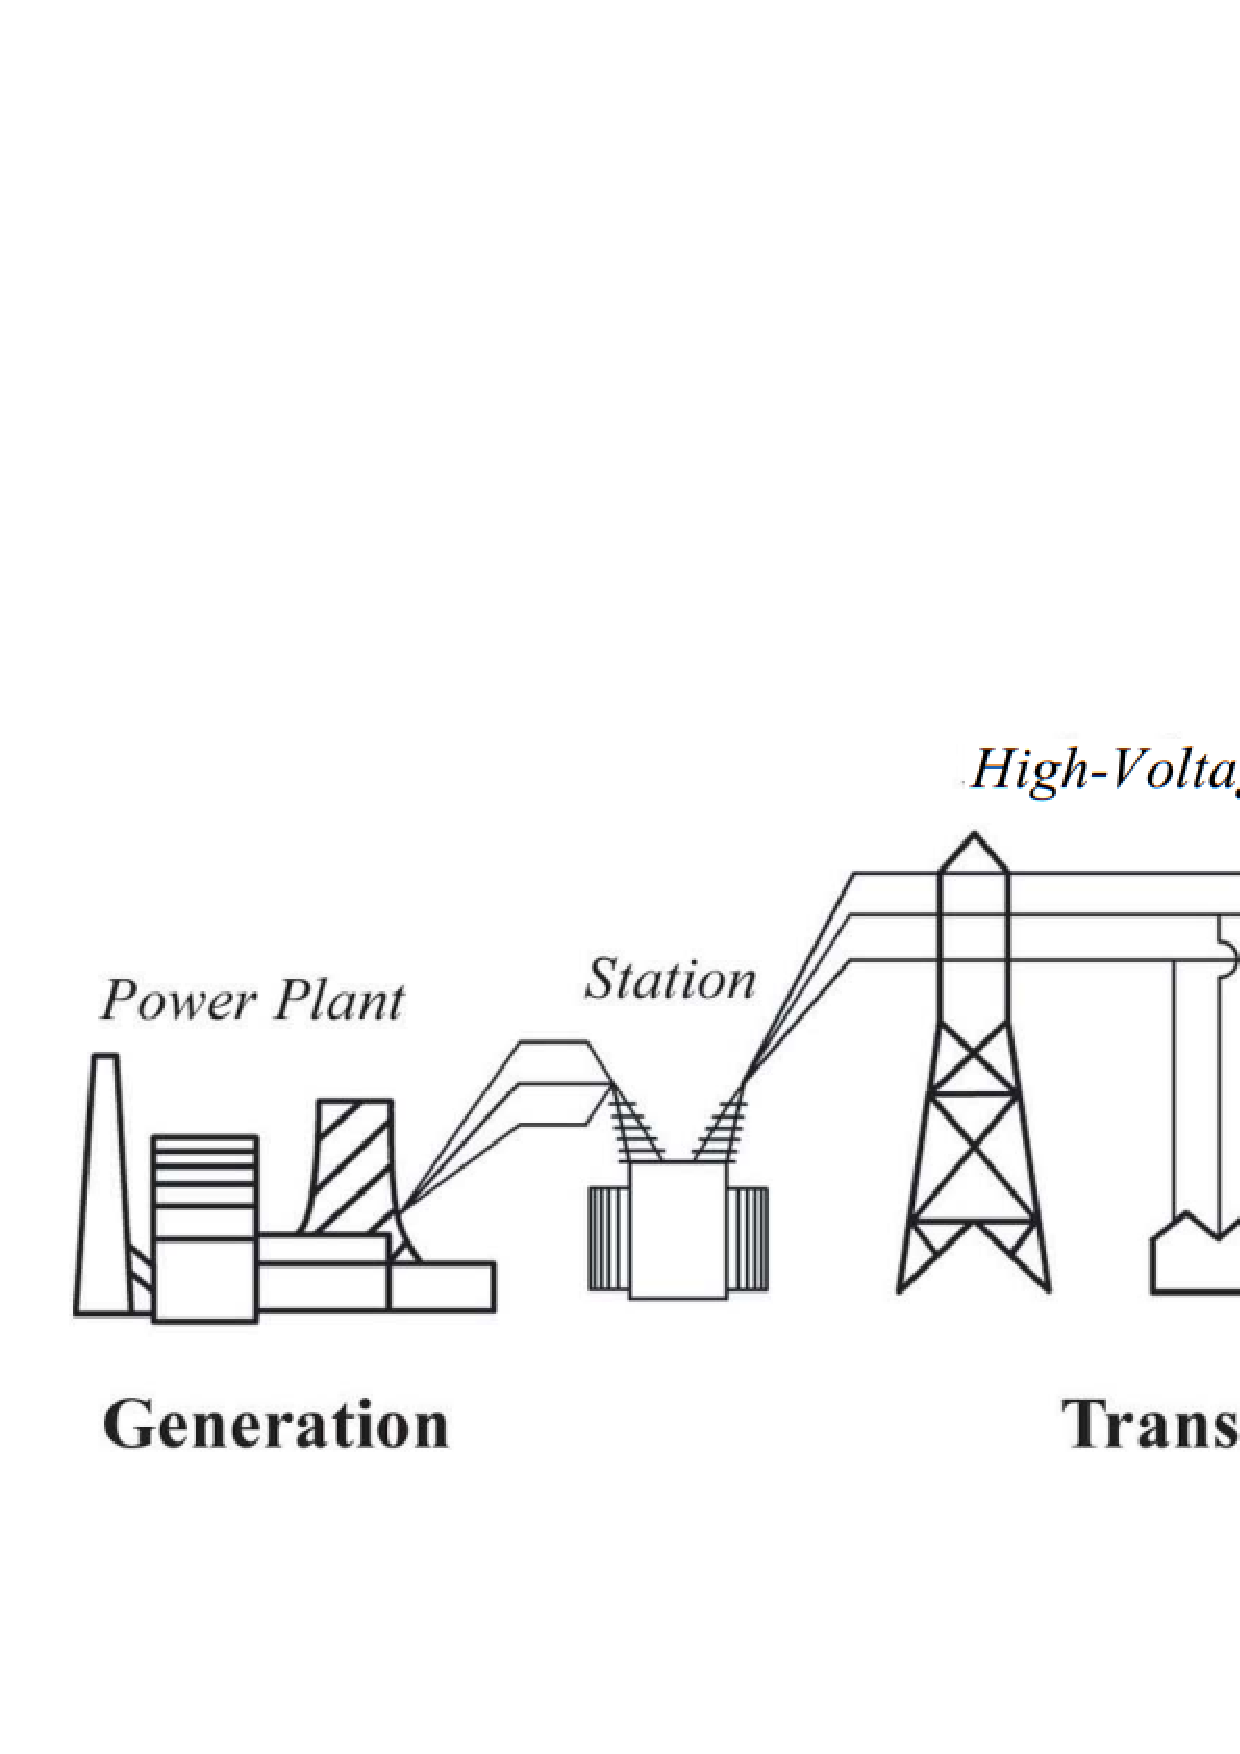
\includegraphics[width=\linewidth]{figures/Blume-PowerGrid-SystemOverView.png}
\caption[Power Grid System Overview]{Power Grid System Overview , as presented in \cite{BlumeStevenW2007Epsb}}
\label{fig:Blume-PowerGrid-SystemOverView}
\end{figure}



\subsection{Overview of the Conventional Power Grid}
The \acrlong{cpg} is a system by which electric power is centrally generated, transmitted, and distributed to industrial, residential,and commercial end users, in order to ensure a reliable access to a sufficient amount of electrical energy. 
\newpage
The \acrlong{cpg}, as described in \cite{BlumeStevenW2007Epsb}, consists of the following subsystems:

\begin{itemize}

 \item The \textbf{Generation Subsystem} which Generates electric power from various sources of energy, to be transmitted for distribution to Consumers. Some examples of installations generating electrical power are nuclear power plants, as well as hydroelectric power plants, feeding water-driven turbines in order to generate power.
 \item The \textbf{Transmission Subsystem} which transmits electric power from the Generation subsystem to the Distribution Subsystem. The current is transmitted via high voltage power lines, minimising energy loss over longer distances.
 \item The \textbf{Distribution Subsystem} which distributes electric power to end users, after converting the high voltage input into lower voltage levels, suitable for consumption.
 \end{itemize}

As described in Chatpter 2.3 of \cite{Rihan2018} %\cite{SmartGridOverview2013}
, the \acrlong{cpg} is facing challenges, related to Black Outs adhering to the increased demands for electrical power . 


%\section{The Smart Grid}
%smart Grid
\section{The Smart Grid}




In order to provide a description of the \acrfull{sg}, a description of the characteristics of the \acrshort{cpg} is provided.





As described in  \cite{BlumeStevenW2007Epsb} by \citeauthor{BlumeStevenW2007Epsb}, some of the characteristics of the \acrlong{cpg} are:

\begin{itemize}
\item Power is generated in real time. In the event a consumer is "flipping a power switch," the power grid must have sufficient resources in order to keep the voltage levels at an acceptable level.
\item The \acrlong{cpg} is controlled by a central management facility known as the \acrfull{scada} subsystem. The monitoring and management of the \acrshort{pg} is initiated from the Control Center, utilising unidirectional communication channels. 
\item The \acrlong{cpg} \acrlong{scada} subsystem is offline, i. e. not connected to any publicly available network. Therefore, operational duties must be performed by personnel physically located at dedicated operational sites.

\end{itemize}

The \acrlong{cpg} originates from the local society-serving power generation facilities initiating the supply of electrical power, which over the years were interconnected to form a grid, connecting consumers to a network of several power generating facilities, providing a more flexible power distribution infrastructure. 


\subsection{Overview of The Smart Grid}


The \acrfull{nist} has published a conceptual model of the smart grid, as shown in 
figure \ref{fig:NIST-SmartGRID-ConceptualModel}.



\begin{figure}[ht]
\includegraphics[width=\linewidth]{figures/NIST-SmartGRID-ConceptualModel.png}
\caption[Smart Grid Conceptual Model]{Updated \acrlong{sg} conceptual model, as presented in \cite[p. 13]{gopstein2021nist}, Figure 4}
\label{fig:NIST-SmartGRID-ConceptualModel}
\end{figure}






The \acrlong{sg} adds Information and Communication Technology (ICT) to the \acrlong{cpg}, in order to transform the  unidirectional communication lines of the monitoring and control infrastructure of the \acrlong{cpg}, into an infrastructure utilising two-way communication between the various parts of the \acrlong{sg} infrastructure. 






%\subsection{The Smart Grid: Critical Information Infrastructure}
%According to \cite[p. 610]{Bîrleanu2019}, the \acrlong{sg} consists of the following subsystems:

%\begin{itemize}
%\item \textbf{the conventional  power grid}
%\item \textbf{intelligent equipment} 
%\item \textbf{communication infrastructure}
%\end{itemize}

%\cite{Bompard2012}...

%...\acrlong{sg} Subsystems
%\begin{itemize}
%\item 
%\end{itemize}




\subsection{The Smart Grid Domains}




The \acrshort{sg} consists of seven domains, as shown in \figureautorefname { }\ref{fig:NIST-SmartGRID-ConceptualModel}:


    \subsubsection{Customer Domain} The customers are the Consumers of Electricity.
    The power infrastructure of commercial or private customers includes \acrfull{ami}, monitoring the amount of energy consumed, both for billing and \acrfull{dr} purposes. Consumers may plan their consumption, avoiding high-cost periods of heavy load, by  selecting time frames of low prices.
    \subsubsection{Markets Domain} The participants of the Markets Domain aims to balance the consumption and demand of electricity, by adjusting prices on electricity. Price adjustments may be used in order to shift consumption from periods of high demand, to periods of low demand.     
    \subsubsection{Service Provider Domain} Services to the Customers,  as well as the Markets and Operators domain, are provided by the Service Provider Domain, fulfilling duties like customer management and billing, as well as a number of emerging services as required. 
    \subsubsection{Operations Domain} This domain consists of Electricity service operators, ensuring efficient and fail-safe \acrfull{sg} operation, by utilising \acrshort{scada} systems and \acrlong{ems}s in order to monitor and control system operational state.  
    \subsubsection{Bulk Generation Domain} The facilities for producing electricity, resides in this domain. In addition to the connection and interaction with  to the Transmission domain, it interacts with the Markets domain, as well as the operations domain.  
    \subsubsection{Transmission Domain} The actors of the Transmission domain aims to reduce energy loss while transmitting a stable and reliable stream of energy from operators in the bulk generation domain to the distribution domain. The market domain provides input on expected level of demand which may require adjustments of the amount of electricity distributed, controlled and monitored by actors in the operation domain.  
    \subsubsection{Distribution Domain} The actors of the Distribution Domain delivers the electricity to consumers according to demand and availability, and monitors generation and consumption data. Bi-directional power-flow is supported. In the case customers have private  power producing facilities, like solar cells and wind turbines, any surplus electricity might be sold, and distributed to other customers.





\cite{2021arXiv210311657E} describes communication protocols in \acrshort{sg}.
\section{Protocols}
A large number of protocols are defined, in order to standardise the operation of the \acrlong{sg}.
A small selection of these, relevant for the scope of the thesis, are described underneath.


\subsection{Time Synchronisation Protocols}
Time synchronisation protocols are controlling the synchronisation of time between various devices of the grid, like the PMUs, collecting phasor measurements from a definde number of measuring devices. Synchronised time is crucial in order to ensure each PMU is able to put the correct time stamp on each phasor measurement, before transmitting the resulting synchrophasor for each time stamp, to the destined PDC device. In the event one of the synchrophasors have an erroneous time stamp, an error affecting the integrity of the synchrophasor data is introduced. As described in \cite{moussa2016security}, \acrlong{ptp} synchronisation network
, as well as \acrlong{gnss} based synchronisation networks, are both capable of producing the precision required by the synchrophasor protocols, as opposed to the more common \acrfull{ntp} commonly used in ordinary computer networks. As my thesis covers \acrshort{ptp} time synchronisation only, my description of time synchronisation protocols is limited to the \acrfull{ptp}.

\subsubsection{Precision Time Protocol}

The \acrfull{ptp} was, as described in \cite{alghamdi2021precision} ...
%\chapter{The Power Grid Control System}
%Control system
\section{The Conventional Power grid control system}
%- SCADA (historical)

%\subsection{The Classic SCADA subsystem}

The \acrshort{scada} system constituted the core part of the control center of the classic \acrlong{pg}, utilising one-directional communication lines in order to manually control and monitor the operational state of the power grid.

Figure \ref{fig:Blume-SCADA-system} shows the main components of the SCADA system.

\begin{figure}[ht]
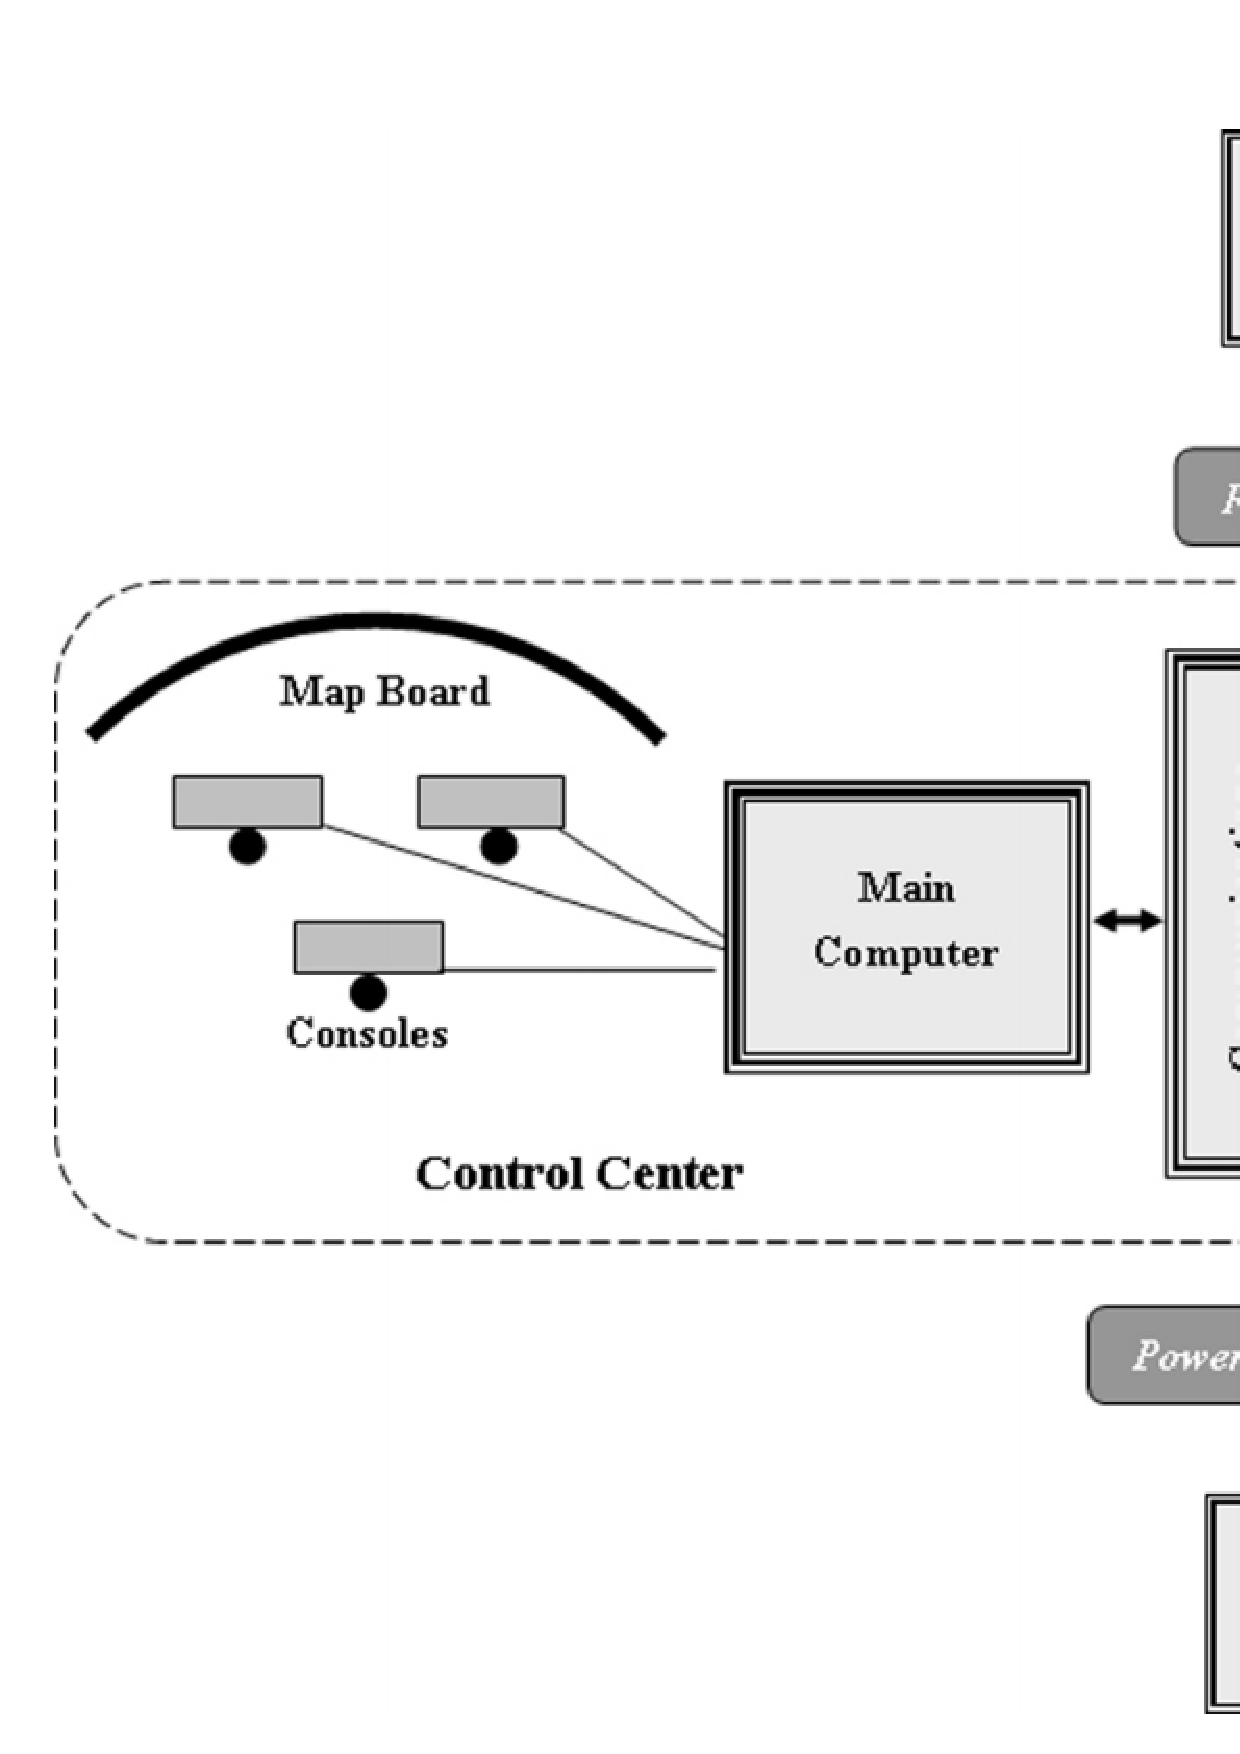
\includegraphics[width=\linewidth]{figures/Blume-SCADA-system.png}
\caption[SCADA system]{SCADA system , as presented in \cite{BlumeStevenW2007Epsb}}
\label{fig:Blume-SCADA-system}
\end{figure}

%[ \fullcite{el2008introduction} ] \\ 


A centrally located control center, optionally being backed up by control centers at one or more locations for redundancy, displays status information from the equipment at the associated substations, received for monitoring purposes. As a response to alarms indicating operational issues, commands enabling remote control of affected infrastructure is issued in order to address the issue, in order to resolve the issue and receive updated status information clearing the alarm. 




%\section{Description}
%- WAMS description

\section{The Smart Grid Control System}


\subsection{Introduction}

Analogous with the modernisation of the classic \acrlong{pg} into the \acrlong{sg}, the \acrshort{scada} subsystem of the \acrshort{pg} is the predecessor of the control system of the modern \acrlong{sg}.
Therefore, a description of the \acrshort{scada} system, evolving from the centralised subsystem controlling the Classic \acrshort{pg}, to the modernised version of the \acrshort{scada} subsystem, initiates the description of the \acrlong{sg} Control System. 




The characteristics of the three generations of SCADA systems% described by \Citeauthor{alcaraz2012security} in \cite{alcaraz2012security},
may be summarised below:
 

 \begin{enumerate}
     \item A Monolithic SCADA system utilises a centralised offline control center  infrastructure, in order to monitor and control the physical system by proprietary control mechanisms.
     \item A Distributed SCADA system utilises a networked, but centralised control  center in order to monitor and control the physical system by proprietary control mechanisms. 
     \item A Networked SCADA system utilises a networked, and online control  center in order to monitor and control the physical system by standardised control mechanisms.
 \end{enumerate}







\subsection{The Modernised SCADA system}
 
 The \acrshort{scada} system is%, as described in \cite{alcaraz2012security},
 a system utilised to supervise and control \acrfull{ci} systems, including \acrshort{pg} infrastructures. Initially designed in order to control physical infrastructure systems like the classic \acrlong{pg}, the Monolithic SCADA system emerged into the Distributed SCADA system. The transition from a Monolithic SCADA system to a Distributed SCADA system transforms, as indicated by %figure \ref{fig:SCADA-CentralisedAndDistributed}
 , the central management center from a centrally controlled mainframe environment, to a networked server environment controlled by operators connected through a \acrfull{lan}
  
  
 The \acrshort{sg} control center emerged from the Distributed SCADA system, into the Networked SCADA system used in order to control modern \acrlong{cps}s, like the \acrshort{sg}.\\ 
 


 





 




However, as explained by \Citeauthor{zamani2020introduction} in \Cite{zamani2020introduction}, the \acrshort{scada} system has a number of shortcomings, making it unsuitable for a \acrshort{sg} enegy distribution monitoring system:

\begin{itemize}
    \item The data polling rate is once every 2-10s, which is not sufficient in order to get real-time measurements.
    \item No time-stamps are attached to samples, making it hard to monitor rate of change over time
    \item State Estimation is not performed with sufficient frequency, if at all.
    \item The ability to observe dynamics is not supported by the system.
\end{itemize}





In order to address these shortcomings, the \acrfull{wams} system\footnote{WAMS is also known as the Wide Area \textbf{Monitoring} System}, described next, was invented.







\section{Wide Area Measurement System}
\begin{figure}[ht]
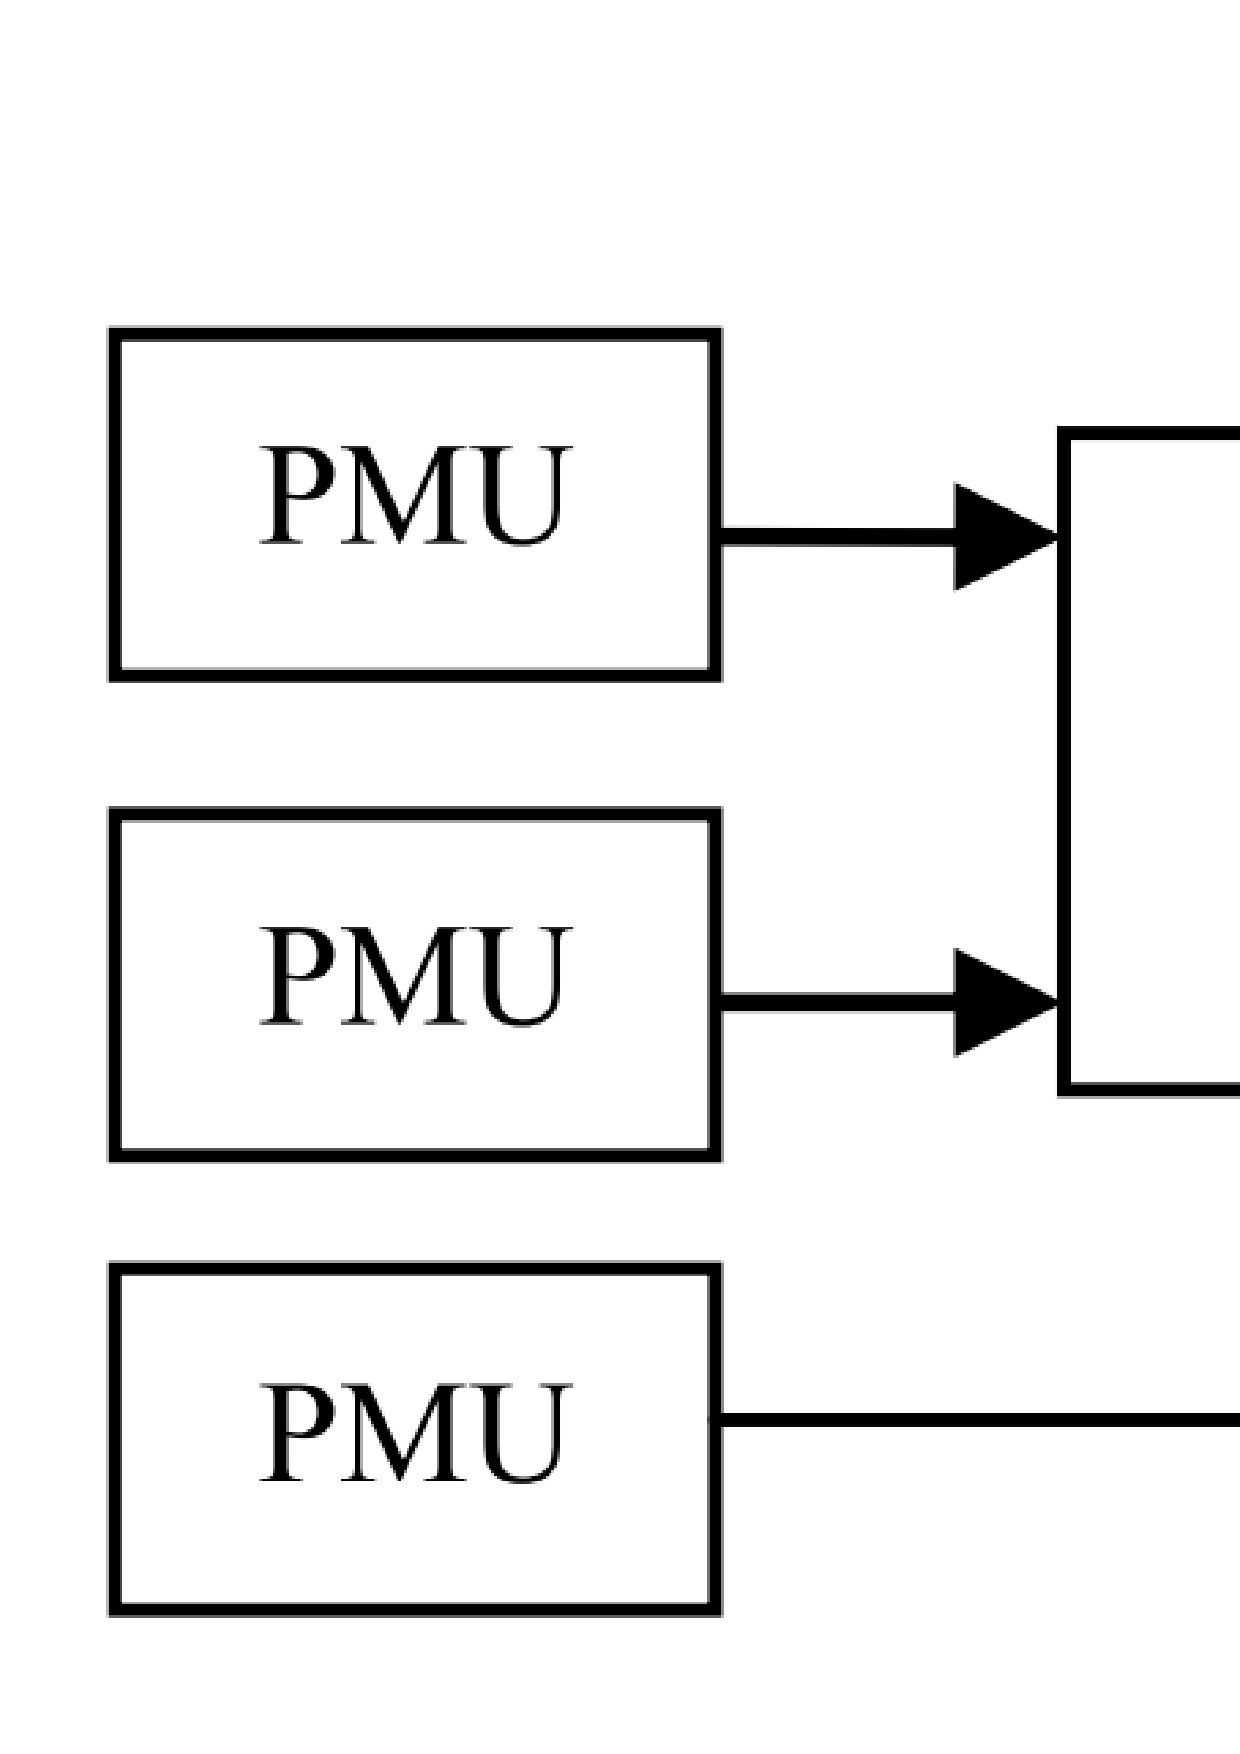
\includegraphics[width=\linewidth]{figures/Kumar-WAMS-architecture.png}
\caption[WAMS architecture]{WAMS architecture, as presented in \cite{kumar2015monitoring}}
\label{fig:Kumar-WAMS-architecture}
\end{figure}

   

In order to ensure the continuous monitoring of the modern \acrlong{sg} energy distribution system, the \acrfull{wams} is utilised. An overview of the \acrshort{wams} architecture, as presented in   \cite{kumar2015monitoring}, is shown as \figureautorefname  { } \ref{fig:Kumar-WAMS-architecture}:

The \acrshort{wams} is, as described in  \cite{kumar2015monitoring}, a  system, consisting of:

(1) \acrshort{pmu}s, (2) \acrshort{pdc}s, (3) The super \acrshort{pdc}, and (4) Communication networks.

The various components might be described as follows, from (4) to (1):
\begin{itemize}
    \item The \textbf{Communication Networks}, providing data transport between \acrshort{wams} components, as required.
    \item The \textbf{Super \acrshort{pdc}} controls several \acrshort{pdc}s constituting a distributed \acrshort{wams}.
\item The \textbf{\acrfull{pdc}} is responsible for collecting and interpreting \acrshort{pmu} measurements, before synchronising the measurements according to timestamps, in order to get more complete status information based on a combination of measurements.
    \item The \textbf{\acrfull{pmu}} is an intelligent measuring device, responsible for registering sensor measurements,  performing calculations like, for instance, phase angles, as well as voltage and current magnitudes. The data registered and processed by the \acrshort{pmu}, is transferred to the nearest \acrshort{pdc}.
    \end{itemize}





\section{Smart grid Monitoring}
The \acrlong{sg} system constitutes a complex system of subsystems, which proper operation is a prerequisite for the successful transmission of electric energy from producers to consumers. 
In order for the \acrshort{wams} to receive status monitoring data, a controlled process for retrieving and transmitting sensor data, is a prerequisite for proper system operation.



\subsection{Description of the Smart Grid  Monitoring system}
Electricity is produced according to the current demand for energy, as controlled by the Demand Management system, dynamically adjusting the energy supply accordingly. In order to successfully reply to the dynamically changing demands for energy, a close monitoring of the production, transmission and distribution of energy is required. In order for the monitoring system to obtain status information, the proper transmission of monitoring data from power status sensors to the   \acrshort{wams}  is essential.


%\section{Storing and transmitting data for monitoring}

\subsection{Phasor Measurene units}

%\subsection{Introduction}

\begin{figure}%[ht]
\includegraphics[width=\textwidth]{figures/phasorMaeasuremantSystems.png}

\caption[Phasor Measurement Systems]{Phasor Measurement Systems, as presented in 

\cite{johnson2018standards} Slide 3

}
\label{fig:PhasorMeasurementSystems}
\end{figure}



\begin{figure}%[ht]
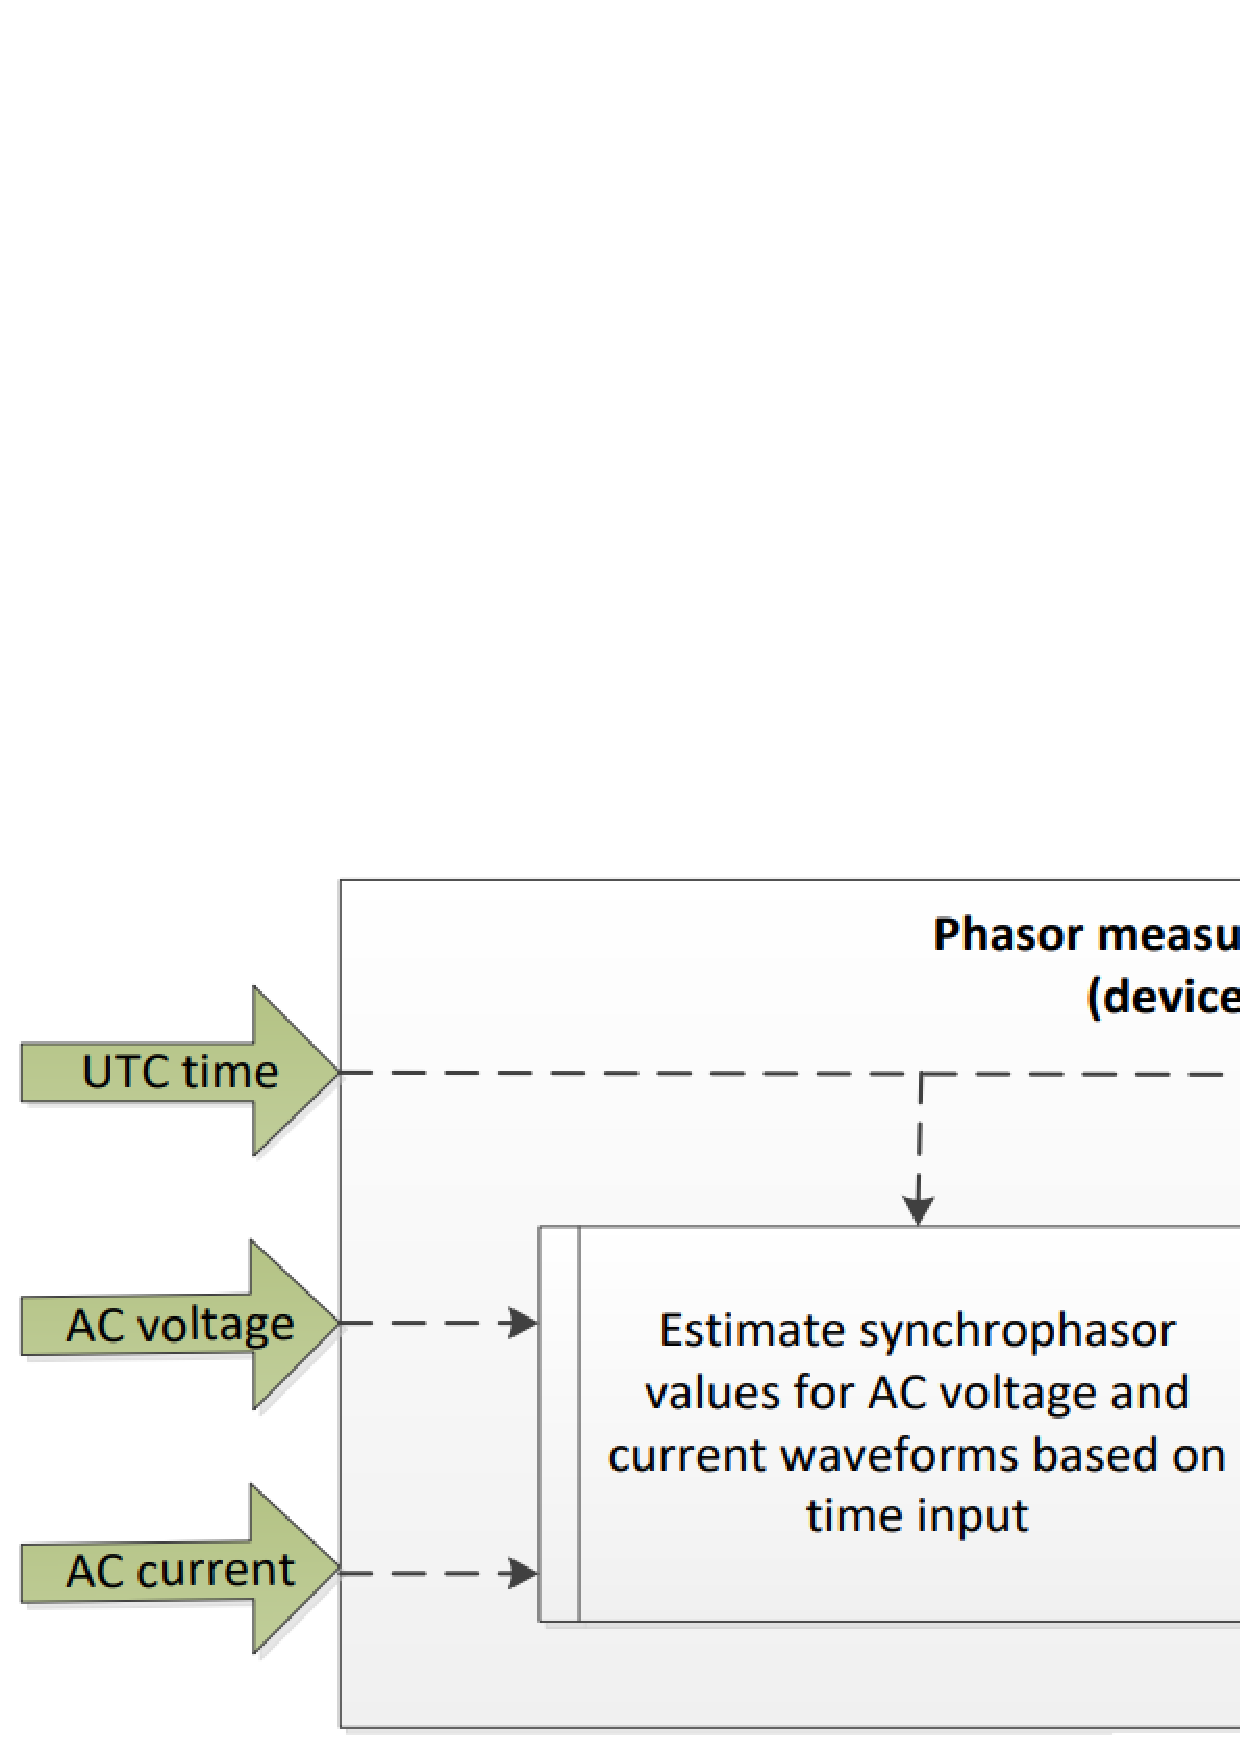
\includegraphics[width=\linewidth]{figures/PMU-in-out.png}
\caption[PMU inputs and outputs]{PMU inputs and outputs, as presented in \Cite[p.12]{iec2018measuring}
}
\label{fig:PMU-in-out}
\end{figure}

\subsection{Phasor data Concentrator}





\
% In \cite{el2018cyber}, \citeauthor{el2018cyber} ...
 


%\subsection{Threats to security}
%In order to ensure the continuous operation of the \acrlong{sg}, identifying security vulnerabilities, and countering threats identified is of vital importance.  




\section{Advantages}
%  - advantages
\section{Security Issues}
%  - security issues
%\subsection{WAMS Security} 

The \acrfull{sg} \acrfull{wams} is a \acrshort{sg} subsystem enabling \acrshort{sg} system operators to monitor the state of \acrshort{sg} energy flow, and general system state. 
A vital requirement for the view of the current state of the \acrshort{sg} energy distribution to be correct is, as described in previous chapters, the ability of the \acrshort{wams} Super \acrshort{pdc}  to utilise synchrophasors collected from the \acrshort{pdc}s to produce a view of the system state. In order for the view to be correct, however, the correctness of the timestamps i critical.  Therefore, in order to produce correct time stamps, the reliability of the Time Synchronisation source is of Critical importance.


\section{State Estimation}

%  - State Estimation: Intro, to explain means to improve grid security.

%\section{WAMS state estimation}
In order to detect abnormalities or errors in the monitoring data received, the \acrshort{wams} includes applications capable of validating the quality of the state information received. Various state estimations exist, some of which give alerts on dubious system state based on comparisons with known good system states. State estimation systems increases the risk of attack detection, thus lowerses the probability of a threat actor being capable of pulling off a stealthy attack.   



%\chapter{Smart Grid Power Flow Monitoring}

%\section{Historical}
%SCADA monitoring flaws -> PMU




%\section{PMUs}
%PMU
%-  Descripton of PMU
%- phasor
%- synchronised phasors
%- Communication with PDC

%\section{PDCs}
%PDC
%- Collecting synchronised phasors from PMU
%- Grouping synchronised phasors with same timestamp into Synchrophasor record
%- At deadline, transmitting Synchronaised phasors, received before deadline.
%- Improved security. 
%\section{Synchrophasors}
%Synchrophasors
%- overview
%- sync precision requirements:
 
%\section{Protocols used for monitoring}
%Protocols
%- Figure from PowerPoint
%- Concentrating on upper left side of figure.


%- capabilities of x.2011 x=synchrophasor protocol

%PTP
%Rationale for concentrating on PTP
%Descriptino of the protocol
%Time synchronisation via PTP
%PTP delay attack (types)

\section{Protocols}
A large number of protocols are defined, in order to standardise the operation of the \acrlong{sg}.
A small selection of these, relevant for the scope of the thesis, are described underneath.


\subsection{Time Synchronisation Protocols}
Time synchronisation protocols are controlling the synchronisation of time between various devices of the grid, like the PMUs, collecting phasor measurements from a definde number of measuring devices. Synchronised time is crucial in order to ensure each PMU is able to put the correct time stamp on each phasor measurement, before transmitting the resulting synchrophasor for each time stamp, to the destined PDC device. In the event one of the synchrophasors have an erroneous time stamp, an error affecting the integrity of the synchrophasor data is introduced. As described in \cite{moussa2016security}, \acrlong{ptp} synchronisation network
, as well as \acrlong{gnss} based synchronisation networks, are both capable of producing the precision required by the synchrophasor protocols, as opposed to the more common \acrfull{ntp} commonly used in ordinary computer networks. As my thesis covers \acrshort{ptp} time synchronisation only, my description of time synchronisation protocols is limited to the \acrfull{ptp}.

\subsubsection{Precision Time Protocol}

The \acrfull{ptp} was, as described in \cite{alghamdi2021precision} ...




\subsection{Synchrophasor Protocols}

The introduction of Synchrophasors in the \acrlong{pg}, 

\subsubsection{Introduction}



As described in \cite{martin2011synchrophasor} and \cite{ali2016performance}, the \acrfull{pmu}, along with the \acrfull{pdc}, were introduced in the 1980s. The communication and data exchange from the PMU to the PDC was standardised by the introduction of the IEEE 1344 standard in 1995, which was the standard communication protocol for synchrophasor data exchange, until the introduction of the IEEE C37.118 in 2005.
The  IEEE C37.118 protocol was derived from the original IEEE 1344 standard, and has undergone a number of revisions, over the years.


In \cite{martin2013synchrophasor}, \citeauthor{martin2013synchrophasor}describes the history of ...

\begin{itemize}
    \item The IEEE C37.118-2005,
    \item The IEEE C37.118-2011
    \item The IEEE C37.118-2018
\end{itemize}




%Unlike the \acrlong{cpg}, the \acrlong{sg} enables bidirectional flow of power, by customers operating micro grids enabling customers to sell excessive power back to the network.



\section{Time Synchronisation}
In order to synchronise the samples received from the \acrshort{pmu}, the \acrshort{pdc}, as well as the \acrshort{pmu} devices producing the samples, is required to adjust their clock by utilising a precise and reliable times source.  Given the distributed nature of the \acrshort{pmu} devices providing samples from locations distributed over a Wide Area Network, the \acrfull{gps} is the  time source selected. 

\subsection{Introduction}


The dependency on networking favors the usage of low-cost \acrshort{gnss} receivers for synchronising time between the growing number of \acrshort{pmu}s deployed at various locations, monitoring energy flow states of the highly distributed \acrshort{sg}. 



\subsubsection{The Importance of Time Synchronisation}

In \cite{dagle2019importance}, \citeauthor{dagle2019importance} states the following aspects as the benefits for Smart Grid operation, of ensuring correct time synchronisation:


\begin{itemize}
    \item  Situational Awareness and Wide-Area Monitoring
    \item  Real-Time Operations
    \item  Power System Planning 
    \item  Forensic Event Analysis
    
\end{itemize}

\subsubsection{Possible effects of Time Synchronisation errors}
Timing errors will, according to ,,, render the data introduced to the \acrshort{wams} system inadequate to enable \acrshort{sg} operatiors to get overview of the Energy supply state of the \acrshort{sg}.

In \Cite{martin2019impact}, \citeauthor{martin2019impact} lists a number of side-effects which could result form the absence of high-quality data material from the \acrshort{wams}.


\begin{enumerate}




    \item Data loss,
    \item Data corruption,
    \item Inaccurate representation of engineering quantities,
    \item Lack of precision,
    \item Incorrect measurement identification,
    \item Excessive or inconsistent latency.

\end{enumerate}

\subsubsection{Precision Time Protocol services}
The \acrfull{ptp} is a network-based time protocol, enabling the time difference between devices to be synchronised within a fraction (in the order of a few $\mu$s) of a second, satisfying the requirements of the \acrshort{sg}. 

\begin{figure}[ht]
    \centering
    \includegraphics[ width=\textwidth]{figures/PTP-timing-Diagram.png}
    \caption[Timing diagram for synchronization messages]{As presented in \cite[p. 51]{Eidson2006}: Timing diagram for synchronization messages.} 
    \label{fig:PTP-timing-Diagram}
\end{figure}  

\subsubsection{Description of PTP time synchronisation}



A device, being synchronised  by the \acrshort{ptp} protocol, reads its system time from a slave clock, being periodically synchronised with a master clock.


The time of the slave clock, is being adjusted according to the following process:


Following the message exchange visualised by \figureautorefname { } \ref{fig:PTP-timing-Diagram}, the Slave clock  uses the time offset from the Master clock time, $offset = [(t_2 - t_1) + (t_4 - t_3)]\div 2$, in order to synchronise with the Master clock. 
In order to be able to achieve the time difference required, the \acrshort{ptp}, as described by  \citeauthor{Eidson2006}, in \cite{Eidson2006}, is dependant on:

\begin{itemize}
    \item Timestamped network events, messages, which is  used for synchronisation.
    \item A method of timestamp transmission as required for synchronisation.
    \item Overcoming any timing impairments introduced by system components.
\end{itemize}




\subsection{Smart Grid Time Synchronisation}



\subsubsection{Introduction}


The \acrlong{sg} is dependant on precise Time Synchronisation, as a Time Synchronisation error of a few $\mu$-seconds may result in \acrshort{sg} instability. The time stamps produced by Synchrophasors, pinpointing the exact time of any system event, is vital in order to ensure precise and reliable system state information.
In the event of a system alert being triggered by erroneous system state Information, corrective actions by operators might have undesired effects. 

\subsubsection[Smart Grid Time Sync Precision Requirements]{Smart Grid Time Synchronisation Precision Requirements}

In order to ensure the time precision required for the \acrshort{sg}, the correct selection of time synchronisation mechanisms is vital. 




\subsection{Synchrophasor}
%\cite{ali2016wide}


%\Cite{rana2015exploring}



The \acrshort{pmu} is receiving values from sensors, on which it is able to calculate voltage level and phase angle of the energy flow. It is utilising a time-source to pinpoint measurements in time, producing synchrophasors, to be transmitted to the nearest \acrshort{pdc}. 

As described by \citeauthor{dagle2019importance} in \cite{dagle2019importance}, the data received from traditional \acrshort{scada} systems are time-stamped after arriving at the control station. The synchrophasors of the \acrshort{wams} on the other hand are, as described by \Citeauthor{ali2016wide} in \cite{ali2016wide}, being time-stamped in real-time before being transferred to the control system. The sampling rate of the \acrshort{pmu}, results in synchrophasor data enabling operators of the \acrshort{wams} to get real-time visualisation of critical elements, like the state of energy flow  of the \acrlong{sg}. The increased granularity of the measurement system allows for the detection of anomalies undetectable by traditional \acrshort{scada} systems, as illustrated by \figureautorefname { }\ref{fig:syncrophasors-vs-scada}. 

The increased sampling rate, of the synchrophasors of the \acrshort{wams} systems enables a more fine-grained view of energy distribution system state changes. However, in order for the \acrshort{wams} system to get the correct system state information, correct time stamps is critical. 
Therefore, the time-synchronisation mechanisms of the \acrshort{pmu} system is of critical importance. \\ 

\begin{figure}
    \centering
    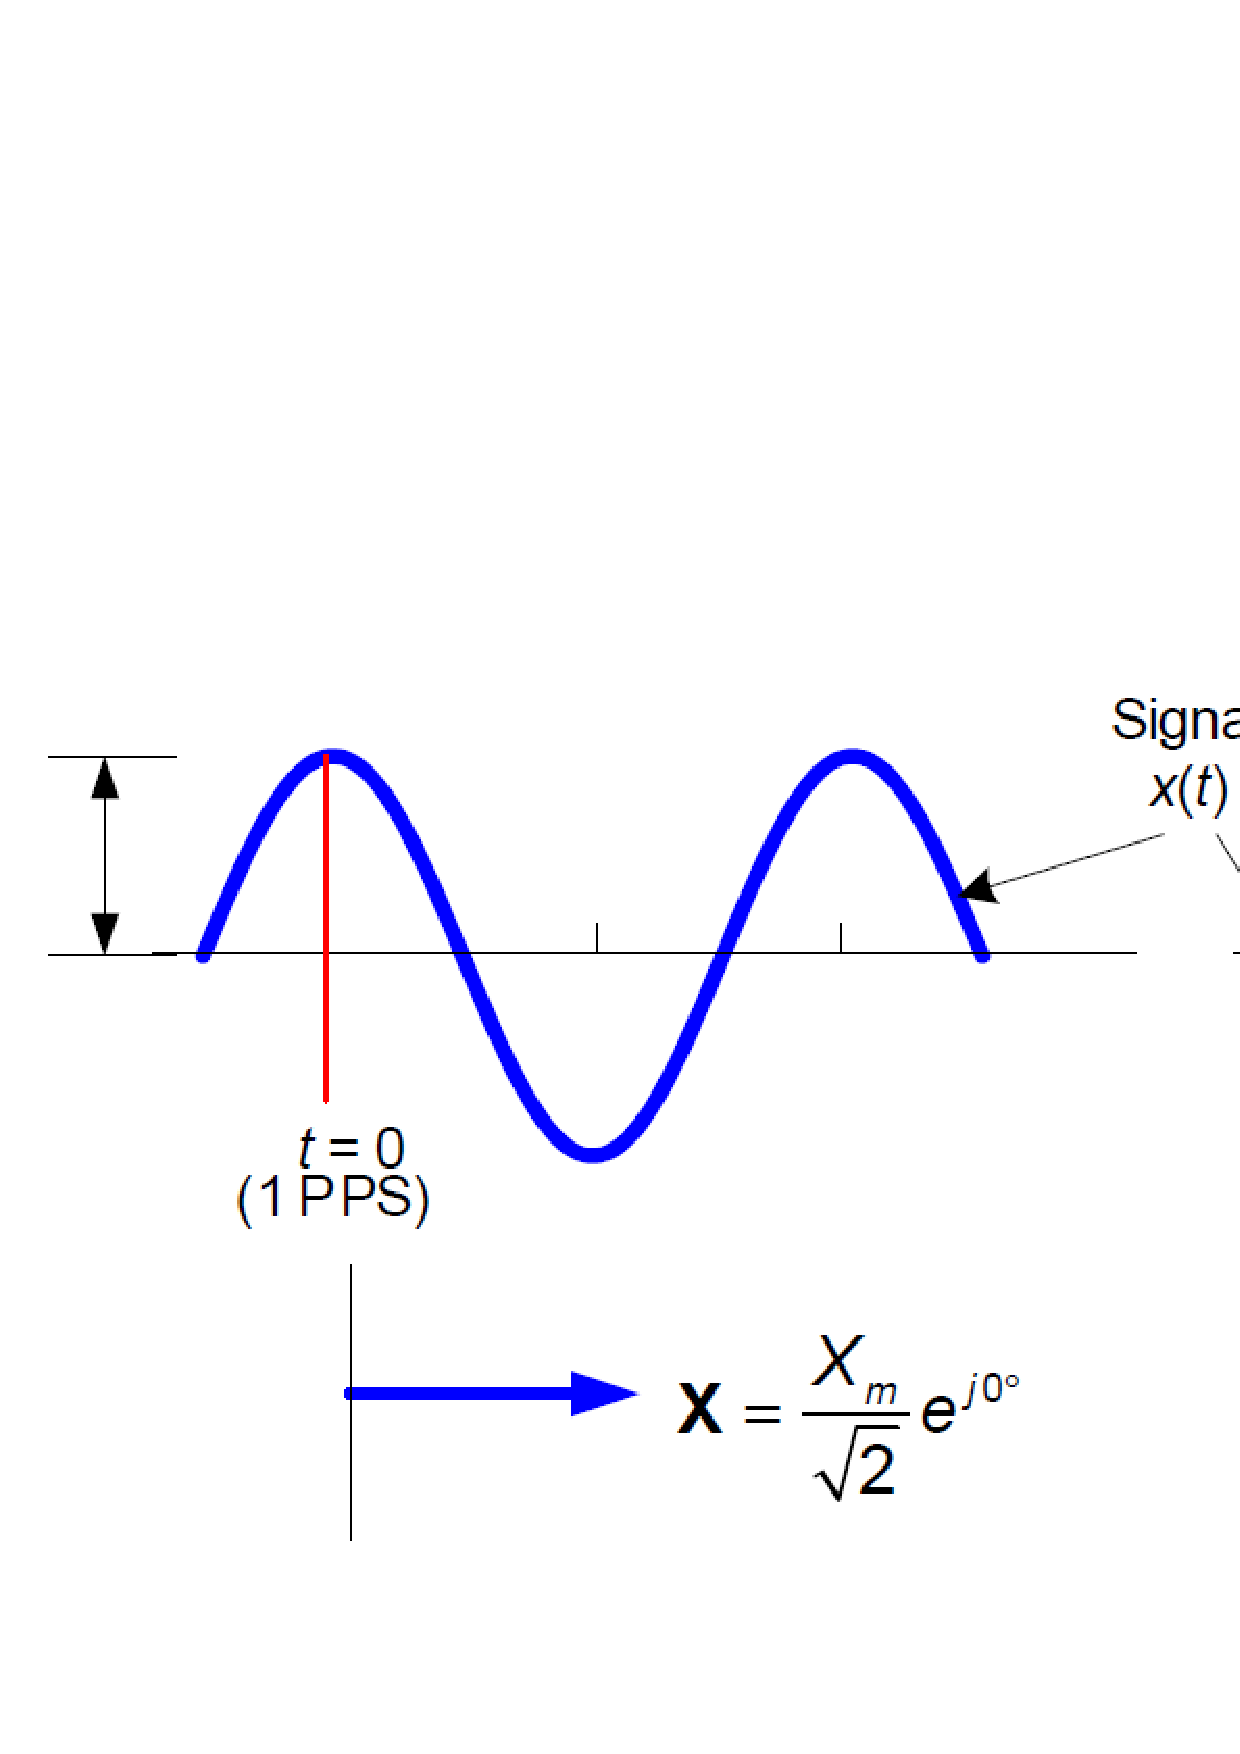
\includegraphics[ width=\textwidth]{figures/Synchrophasor-Definition.png}
    \caption[Convention for synchrophasor representation]{As presented in \Cite{schofield2018design}: Convention for synchrophasor representation.}.
    \label{fig:Synchrophasor-Definition}
\end{figure}  

%



\chapter{Smart Grid Cyber attacks}
%Overview of cyber attacks
%\section{Threat Actors}
%Threat actors
%- Threat actor Categories
%  - MitM
%  - MotS
%- Threat actor Capabilities

%\section{Types of Cyber Attacks}
%Cyber Attacks
%- Cyber Attack Categories
%  - (D)DoS
%  - FDI
%  - Time Delay Attack
%  - Malware





%\chapter{Cyber Attacks on the Smart Grid}









The \acrfull{sg} is a complex system delivering electrical power to a society more dependant on electricity then ever, given the transition from traditional sources of energy to electrical energy on areas like agriculture, industrial production, heating, and more recently, transportation.
The transition of the electrical grid from the classic \acrlong{pg} to the \acrlong{sg} exposed, as previously described, the \acrlong{ci} of the power grid to attacks from remote locations via the Internet.

Before focusing on smart grid time delay attacks, an introductory overview of a selection of other cyber attacks targeting  the smart grid will be given.



\section{An introduction to Smart Grid Cyber Attacks}


\section{Attack via time protocols}

Computer systems reachable\footnote{Systems could ultimately be targeted utilising USB sticks, if not accessible from the Internet.} from the outside world,  are potential targets of Cyber attacks. The eventual recoveries of the initial Cyber Attacks was followed up by defence actions, resulting in more advanced attack techniques, has evolved to a continuous battle of control between attackers and defenders. \\


There are numerous Threat Actors of various skill levels, from so-called "Script Kiddies" to professionals, aiming to get unauthorised access to systems, for fun, fame, or for more serious reasons, like terrorism or financial gain. 
subsubsection{Attacker Types}

\begin{itemize}
    \item The \textbf{Internal attacker} has privileged access to, at least parts of, the internal infrastructure of the target, enabling the ability to take malicious actions not available to non-internal attackers.
    \item The \textbf{External attacker} is limited to attacking the targeted infrastructure from the outside, typically through network connections.
    \item The \textbf{Traffic Injector attacker} adds network packages to the benign traffic of the networks of the target, in order to produce the desired effects on the state and operation of the targeted infrastructure. 
    \item The \textbf{\acrshort{mitm} attacker} interrupts the communication between the two parties A and B, impersonating as B to A and vice-versa.
    \item The  \textbf{\acrshort{mots} attacker} are able to eavesdrop on communications, without any privileged access to enable the direct modification of any data transmitted.
\end{itemize}



The various types of attackers possesses various malicious action capabilities, which they may use in order to attack their intended target in numerous ways.


\subsubsection{Advanced Persistent Threat (APT)}

The most advanced, sometimes stealthy, Cyber Attacks are imposing an imminent uncertainty amongst those tasked with the safe operation of critical systems like the \acrshort{sg}. Threat Actors capable of breaking in to presumably secure critical systems, staying undetected for several months or years, constitutes a persistent threat to the secure operation of the system.

\subsection{Time  Protocol Threats}








\
\subsubsection{Attack Types}
As described in \cite{ullmann2009delay}, a number of threats affecting the \acrshort{ntp} and  \acrshort{ptp} time protocols is observed:



\begin{itemize}
    \item Grand Master Time Source Attack
    \item \acrfull{dos} attacks: Specialised protocol-specific \acrshort{dos} attacks, as well as traditional IP-based \acrshort{dos} attacks.
    \item Cryptographic Performance Attacks
    \item Packet Manipulation Attacks
    \item Spoofing Attacks
    \item Replay Attack   
    \item Rouge Master attack 
\end{itemize}



\subsection{Examples of Cyber attacks}
As described in \cite{sundararajan2019survey}, a number of security incidents targets the \acrshort{sg} specifically, like the 2015 BlackEnergy3 attack on the Ukranian  Power Grid, the StuxNet worm of 2010, as well as the watering-hole remote access trojan attack of 2014. 
Any online \acrshort{sg} infrastructure containing vulnerabilities, is equally inflicted by attacks not specifically targeting \acrfull{sg} like the WannaCry ransomware cryptoworm of 2017, targeting the EternalBlue vulnerability of unpatched windows computers.\\ 



\subsection{Attacks targeting the control systems}


\acrfull{dos} attacks, is identified by several papers, like  \cite{sundararajan2019survey} and \cite{gupta2017survey} as  a threat to \acrshort{sg} availability. \\ 

%In addition, occurrences of the \acrfull{tsa}, sending modified \acrshort{gps} timing information to various control systems, has proven to be a real threat to \acrshort{sg} operation, as described  in \cite{ZhangTimeSync2013}. \\ 







%\subsubsection{Time Synchronisation attacks}
\section{Cyber Attacks targeting Smart Grid}

The two-way communication lines of the\acrlong{sg} systems opens the possibilities of communication between the networks of energy distributors and the networks of consumers, serving purposes as automatic measurement of energy consumption, as well as dynamic adaption of energy production according to variations in demand for energy over the hours of the day.
The transition from networks managed by closed communication channels to networks communicating over IP-based networks, exposes\acrlong{sg} networks to Cyber attack vulnerabilities.



Malicious threat actors having privileged access to the infrastructure, is able to perform various kinds of internal attacks. Traditionally, anyone aiming to attack the \acrlong{pg} infrastructure, was obliged to get physical access to the premises, from which the infrastructure in question was controlled. Following the transition to the online \acrshort{sg}, the network connecting the grid to the outside might be utilised in order to execute any Cyber attack requiring internal privileged access from the outside.


\subsection{External Attacks}
External attacks is characterised by malicious actors attacking the infrastructure from the outside, without having the privileged access required in order to target internal system vulnerabilities.




\subsubsection{Denial of Service (DoS) Attack}

%\subsubsection{GNSS Spoofing attacks}

\subsection{Internal Attacks}
The distinction between external and internal attacks, is the level of access required in order to perform the attack in question.

\subsubsection{Man in The Middle (MiTM) Attack}



\cite{itkin2017security} provides information on \acrshort{ptp} delay attacks.





\section{Types of PTP delay Attacks}
Several attacks which targets the \acrlong{ptp}  utilises vulnerabilities 



As described in \cite{ullmann2009delay}
\subsection{Put all clocks back}

\begin{equation} \label{DSM}
    D_{prox}=D_{SM}\frac{1+d}{d},d>1 
\end{equation}
\subsection{Put specific clock back}
\begin{equation} \label{DMS}
    D_{prox}=D_{MS}\frac{1+d}{d},d>1 
\end{equation}

\cite{finkenzeller2022feasible}
%\chapter{Method} 

%The method chapter should describe in detail which activities you undertake to answer the research questions presented in the introduction, and why they were chosen. This includes detailed descriptions of experiments, surveys, computations, data analysis, statistical tests etc.

\section{Introduction}




The aim of the thesis, is to investigate to which degree a stealthy time delay attack on \acrshort{pmu} data may be successfully  executed. \textbf{Some papers} describes a number of varieties of the PTP delay attack, while \textbf{other papers} describes the attack to have severe consequences to the \acrshort{sg} infrastructure. The primary goal of the actual attack is to stay undetected, while exposing the infrastructure under attack to an attack having the most severe consequences possible, while still avoiding detection.  In a preliminary phase of the attack, a phase of attack simulation will provide useful information, aiming to learn more about detection probability, as well as some empirical background for the evaluation of possible consequences.
The potential outcome of the simulation may be used in order to prepare for attacking the actual infrastructure with attacks with a low attack detection probability and, to the best possible knowledge, with foreseeable consequences of the attack.\\ 


As part of the introductory studies of the topic selected, a couple of searches on the NTNU literature search facilities returned a number of books, like \cite{BlumeStevenW2007Epsb}, \cite{kabalci2019smart}, and \cite{momoh2012smart}, covering introductory chapters on Power Grid and Smart Grid. The introductory chapters heavily relies on descriptions from relevant book chapters. 


%For the \acrfull{wams} Security parts, a small number of surveys, as well as a collection of papers are investigated, covering  synchrophasor protocol attack vulnerabilities, highlithing some known side effects of successful synchrophasor protocol attacks. The introductory brief coverage of \acrshort{sg} security, is followed by a coverage of common synchrophasor protocols, focusing on attack vulnerabilities of the protocols covered. \\ 






%Several test cases utilising PMUs and PDCs



%In order to investigate, systems like mininet. \\ 


\section{Research Design}
%This section will inform the reader of the NATURE of your study. In other words, broadly speaking: are you aiming to describe a phenomena (descriptive design), are you aiming to explore a topic (exploratory design), are you looking to identify causal relationships between factors (causal design)?

%The aim of the thesis, is to present an overview of concepts, as well as to to provide examples from the literature related to the Smart Grid WAMS being vulnerable to attacks on the Synchrophasor protocols. 
In order to be able to observe the effects of exposing a \acrshort{pmu} to a time delay attack, the real attack is dependant on getting access to expensive equipment, like a \acrshort{pmu} as well as the interconnected infrastructure.
As previously discussed, a time delay attack on Synchrophasors imposes a high risk of causing damage to the infrastructure targeted.
Given the high potential for damage, a good option for visualising any potential effects a time delay might have on the values produced by a \acrshort{pmu} under attack, would be to simulate the attacks.
There exists a number of projects which utilises MATLAB and SIMULINK in order to model power grid components in general and, specifically, \acrshort{pmu}s.



In order to 

Based on the findings of the initial literature study concerning vulnerabilities, the literature study continues providing potential scenarios for stealthy MiTM attacks on the synchrophasor transmission system, investigating the success of the attacks maximising side effects while minimising the probability of being detected.

As the final part of the thesis, a theoretical discussion, aiming to provide answers to the research questions, will be conducted.\\ 

\textbf{TO DO:}
\textit{As a experimental part of the thesis, possibilities of testing one or more detection and mitigation techniques might provide a contribution to the final discussion and conclusions based on my own experimental results}


\section{Research Methods}

%Following the description of your research design, you should also devote a section to describing the research methods you applied during your study. Each design will provide you with many possibilities of methods to use.

In order to provide theoretical evidence on which to answer the research questions, a literature study will be conducted.
For any experimental results, experiments will be described, implemented and executed.

\section{Measurements}

%Once you clarified the method you used, it is time to explain exactly WHAT you measured (e.g. service quality, brand image, satisfaction, purchase intention) and HOW you measured

Vulnerability to time-shift attacks are quantified by articles describing theoretical aspects of the mechanisms for the calculation of valid time-stamps, and the inherent tolerance level for calculation errors. Modern Smart Grids require the time deviating from the correct time by a fraction of a millisecond. Specifically, according to \cite[p.  1953]{moussa2016security}, the allowed time deviation for a 50Hz electrical system\footnote{As used in Norway, for instance} must be within $\pm$31.8 microseconds, in order to adhere to the 1$\%$ \acrfull{tve} requirement, as specified by the  IEEE C37.118 standard. \\ 

Experimental investigations reported by articles selected will be provided as relevant examples, in order to support any discussion arguments for the purpose of reaching conclusions.  

\section{Sample}

%In this section you should detail (at least!) the population of your study, your sampling technique (which technique you used to select the people who took part in your study) and how you established your sample size.
The samples for my literature study will be papers relevant for the discussions, in order to provide answers to the research questions.\\ 

Any execution of experiments will provide experimental samples, with the aim of supporting discussions and conclusions.
\section{Validity and Reliability}

%Now, here is a SUPER important section that 99\% get wrong(I completely made up this figure, simply because I want to convey a point!). Validity (that you measured what you intend to measure) and reliability (that the measurements used, such as your scales, are consistent and replicable) are two concepts that simply have to be addressed and have to do with your measurements.
In order to increase the validity and reliability, a number of articles will be included as the foundation for any conclusions. My personal selection of papers deemed relevant for my discussion, will be selected highlighting on articles being included as relevant articles by survey papers, as well as papers gaining a high relevance score on literature search sites.\footnote{... like the NTNU ORIA site (\url{https://innsida.ntnu.no/litteratur}).} Another selection criteria aiming to increase validity and reliability will be a focus on selecting articles receiving a high number of quotations ratings on sites like Google Scholar. %First and foremost, though, a sound and critical validation of the relevance for the questions at hand is still mandatory. \\  



For the experimental parts, my project is utilising a selection of PDC and PMU simulator packages. In order to validate the phasor data generated, the included validation capabilities of the simulator packages are utilised.

\section{Infrastructure used during experiments }
\textbf{TO DO:}
\textit{A selection of a relevant infrastructure for experiments will be made according to  specific needs and availability.  }\\ 

In order to provide practical results on which to base the discussions and conclusions, the following tools will be utilised;

\begin{itemize}
%    \item The iPMU suite, including iPDC, iPMU and PMUSimulator, running on virtual Ubuntu Linux instances
%    \item The pyPMU suite, including tinyPDC, tinyPMU and , running on virtual Ubuntu Linux instances \cite{vsandi2015python}, \cite{vsandi2016pypmu}
    \item A SIMULINK model, downloaded from \textbf{URL} is used as the basis for the simulations.
    \item MATLAB, \textbf{latest version}, with SIMULINK added, is used for running the simulation. 
    \item The SIMULINK DSP and MATLAB Digital Signal Processing toolkits are required in order to run the simulations.
    \item The \textbf{Model inspector} functionality is used in order to compare the delayed ouput to the original one.
    \item A Windows 10 laptop is being used for the simulations
    
 %   \item mininet will be utilised for networking
 %   \item Wireshark will be utilised for synchrophasor packet analysis
 %   \item Python will be utilised in order to visualise the results

\end{itemize}

%\section{Instruments or Equipment}

%Sometimes, especially in causal studies when researchers are developing experiments, it is important to detail the instruments or equipment that were used in the study.



\section{Simulating a Time Delay attack}



\subsection{Scenarios}

For the experimental part of my thesis, a number of attack scenarios will be required. The aim is to investigate various attack vectors which might be used by a sophisticated man-on-the-side threat actor in order to execute an attack while staying undetected. 

\subsection{Background} 

A number of assumptions is stated, in order to narrow the scope of the thesis.

\subsubsection{Attacker policy assumptions}
A sophisticated threat actor would most likely want to avoid detection by anyone protecting the targeted infrastructure.
Therefore, executing an attack which may be detected should be avoided at all costs.
As a consequence, any decisions related to actually executing the attack should be as a result of promising results following a stealthiness assessment process\footnote{Simulations of possible effects could be part of a stealthyness assessment process}. 

\subsubsection{Attack Prerequisites}
A stealthy attack with small impact is preferred over an attack having more severe impacts, at a higher risk of detection.
The ideal attack would be an attack having maximal impact on the target, while the risk of detection being minimal. 


\subsubsection{Attack design challenges}
A part of the challenge would be to design an attack producing a high impact on the target, while staying undetected.

\subsubsection{selected approach}
One possible solution could be to determine the minimal efforts needed in order to execute an attack with a high probability of producing the effects desired, while keeping the attack detection probability low.



\subsection{Definition of scenarios}
In order to provide experimental results in order to answer the Research Questions stated, a number of attack scenarios are defined.

The main method of simulation would be a delayed forwarding of values, where a specified delay $d$ is applied to the PMU input, replacing any sample $s(i)$ with the sample value $s(i-d)$, simulating clock drift, producing effects similar to a \acrlong{tda}.

The simulation could be performed using a number of delay functions, for instancs:
\begin{enumerate}
   
\item  Exposing the targeted PMU to a constant delay, from a specified initiation time.
    The delay is switched on, unaltered from the time of initiation, for the duration of the simulation. 
\item  Exposing the targeted PMU to a constant delay for a limited time, from a specified initiation time, switching it off during the simulation.  
\item  Exposing the targeted PMU to a increasing delay for a limited time, from a specified initiation time, switching it off during the simulation.   
\end{enumerate}
    


\subsection{Attack Implementation}
%The attacks would be implemented as MATLAB functions executing attacks on targets implemented as SIMULINK simulations. The various scenarios would  be required to be sufficiently similar to be implemented as variations of a single attack framework, in order to avoid the need of creating more than a single attack framework.     

%In order to prepare for attacks, a plan might be to implement the techniques described in \cite{gilad2014off}.



%\textbf{\cite{barreto2016undetectable} proves the requirement of exposing more than two PMUs to a delay attack, for the attack to be undetectable.}




A number of physical investigations related to the effects of any intended attacks on the intended targets, would increase the knowledge of a potentially complex target, increasing the probability of staying undetected during the attack. In order to avoid exposing expensive and critical power system infrastructure to physical damage or downtime,\footnote{In a test lab environment, downtime could be acceptable, whereas the risk of physical damage of typically expensive equipment may be too high, at least not in the initial phases of investigations.} such practical investigations would preferably be performed in a simulation environment.

\section{Creating a Simulation environment}

This approach could be taken by a threat actor during a phase of investigations in the preparation of the actual attack, for the purpose of learning more about the possible consequences of performing intended actions on the intended target. One of the most important priorities of the threat actor, is to stay undetected for as long as possible. Simulations are designed in order to investigate the selected attack scenarios. The planned attack is implemented using a combination of Simulink and MATLAB. The execution of each simulation will produce corresponding graphs, illustrating any visible effects the attack may have on the system, by analytically comparing the output produced by the attack, with the alternative output of the unmodified, and correct Synchrophasor signal corresponding to  a situation of no attack being performed.

\subsection{Modelling a PMU}

As the plan of the threat actor is to expose  a number of \acrshort{pmu}s to a time  delay attack, the plan is to build a model of a \acrshort{pmu}, allowing the model to be run while altering any time stamp values required, in order to investigate any observable effects on the output from the \acrshort{pmu}.
 \begin{figure}[ht]
\centering
\includegraphics[width=\textwidth]{figures/SimPMU.png}
\caption[PmuSIM SIMULINK model]{A SIMULINK model for the simulation of PMU time delay attacks}

\end{figure}



\subsection{Experimental Procedure}
%\textbf{TO DO:} \textit{Describe experimental procedure, dependant on experiments and experimental environment selected.}.
In order to complete one iteration of the simulation, each step should be completed, as required.
\begin{enumerate}
    \item Start Matlab
    \item Open a MATLAB script, to be specified.
    \item Inspect and modify a selection of variables, and execute the script for each run. The script will produce:
    \begin{enumerate}
    \item Output data logged to workspace according to the model.
    \item One figure for each of the PMU components "Angle", "Frequency" and "Magnitude".
    \item The figures are stored as specified in the MATLAB script.
    \end{enumerate}
    \item Planned analysis is to be determined. 
\end{enumerate}
Assumptions: 
Focus on a few optional tolerance levels. One Option: Assume a similarity of 0.95 to be hardly detectable.  
\begin{itemize}
    \item Use the Simulation Data Inspector for graph comparisons.
    \item Compare the original/native signal with the delayed version, by tolerance level.
    \item Tolerance levels: $1\% (0.01)$, $5\% (0.05)$ and $10\% (0.1)$ 
\end{itemize}

\begin{enumerate}
    \item The green portion of the line indicates signal similarity, indication periods with a low probability of attack detection.
    \item The red portion of the graph is to be interpreted as time periods where the attack detection risk is too high for the attack to remain stealthy for lengthy periods of time.

\end{enumerate}
\subsection{Definition of Experiments} \label{sec:ExpDef}

%As discussed in an \textbf{Earlier Chapter}, according to \textbf{SELECTED PAPERS}, the \acrshort{sg} \acrshort{se} systems analysed would detect attacks producing signal differences of various levels of similarity. %around $10-15\%$ similarity.





The experiments will focus on various levels of assumed detection thresholds.

My experiments will cover a selection of attack strategies for the selection of threshold levels of $1\%$, $5\%$ and $10\%$ similarities.

\begin{itemize}
    \item Square pulse signal: off, constant-delay, off
    \item Increasing delay, drop to 0 before simulation end
    \item Increasing delay, decreasing to 0 before simulation end
    \item Constant delay: dela on for the duration of the simulation
\end{itemize}

The current figures of chapter \ref{chap:Results} are produced by exposing the PMU to a square pulse delay.
%




%The experiments, therefore, will focus on levels of delay of 0.1 to 0.15. For each level, the analysis will focus on various attack strategies, reaching the delay level in 1,2,3 and 4 steps, before keeping the delay for a total duration of  5 to 15 seconds.

%The experiments will be performed utilising \acrshort{pmu} simulation software, utilising available verification tools to ensure the compliance with established standards like the <--->
%The plan is to recreate experiments performed by <----> in a live environment, utilising  In order to test mitigation, mininet will be utilised

%Generate PMU data utilising simulators verified for compliance


%Utilise SADF \cite{SADF-framework} in MATLAB.

%Once again, in case you are running a causal study and an experiment, it is important to detail the experimental procedure.

%Explain, to the reader for example, what was the experimental task (what did the participants have to do?), the extraneous variables that were controlled (variables of the environment that could affect the cause and affect relationship).





%\let\includegraphics\includegraphicsold

\chapter{Results} \label{chap:Results}

%The results chapter should simply present the results of applying the methods presented in the method chapter without further ado. This chapter will typically contain many graphs, tables, etc. Sometimes it is natural to discuss the results as they are presented, combining them into a `Results and Discussion' chapter, but more often they are kept separate.\\ 

The following sections presents the results for each attack type, with subsections for the detection threshold levels selected, as defined in section \ref{sec:ExpDef} \\ 

Comments on the results are deferred to chapter \ref{chap:Discussions}
\newpage
\section{Ascending delay function}
\begin{figure}[hb]
 %   \includegraphics[trim=2 10 14 4, clip]{figures/v_AllFig-DelayOf_2-Ascending.png}    
    \includegraphics[width=0.95\textwidth]{figures/v_AllFig-DelayOf_2-Ascending.png}    
    \caption{Ascending delay combined output}
    \label{fig:simPMU-allfig}
\end{figure}


     \begin{figure}
        \caption{Component-wise output}
 
    \includegraphics[width=0.95\textwidth]{figures/v_MagFig-DelayOf_2-Ascending.png}    
         %\caption{magnitude Output}
         \label{fig:AscMag}
   \includegraphics[width=0.95\textwidth]{figures/v_AngFig-DelayOf_2-Ascending.png}    
          %\caption{Angle Output}
         \label{fig:AscAng}
   \includegraphics[width=0.95\textwidth]{figures/v_FreqFig-DelayOf_2-Ascending.png}    
         %\caption{frequency Output}
         \label{fig:AscFreq}
 
\end{figure}















%\section{off, on, off: abrupt}
%\subsection{Findings for a detection threshold level of 0.01}
%\subsection{Findings for a detection threshold level of 0.05}
%\subsection{Findings for a detection threshold level of 0.10}

%\section{increasing, on , decreasing: small steps}
%\subsection{Findings for a detection threshold level of 0.01}
%\subsection{Findings for a detection threshold level of 0.05}
%\subsection{Findings for a detection threshold level of 0.10}

%\section{increasing and continuous}
%\subsection{Findings for a detection threshold level of 0.01}
%\subsection{Findings for a detection threshold level of 0.05}
%\subsection{Findings for a detection threshold level of 0.10}

%\subsection{Findings for a detection threshold level of 0.01}
%\subsection{Findings for a detection threshold level of 0.05}
%\subsection{Findings for a detection threshold level of 0.10}
%\section{Findings for delay level 0.11}
%\section{Findings for delay level 0.12}
%\section{Findings for delay level 0.13}
%\section{Findings for delay level 0.14}
%\section{Findings for delay level 0.15}



\chapter{Discussion} \label{chap:Discussions}


%Here you should discuss all aspect of your thesis and project. How did the process work? Which choices did you make, and what did you learn from it? What were the pros and cons? What would you have done differently if you were to undertake the same project over again, both in terms of process and product? What are the societal consequences of your work?

\section{Introduction}


\subsection{Verification of model}

For verification purposes, results for the delay level of 0 is presented.  In this case, the original and delayed graphs should be identical.
\subsubsection{Comments on the result:}
The results of running the simulation with a delay of Zero produces a number of figures of pMU output consisting of indistinguishable signal graphs for the Native and Delayed output, with identical standard deviation, and no traces of red parts in the graphs showing degree of tolerance, for any \acrshort{pmu} output Component under study. The result may be regarded as indicative of a correctly working delay function, as well as the dualPMU being a correctly designed PMU subsystem. 




\section{Comments on various aspects related to the results}

Discussion of results related to expected results, according to theoretical conclusions.





\subsection{Similarity Requirements}
In Figure \ref{fig:VoltageInstantDelayOne} (see above), for a similarity of 5\%, the attack detected  at level 1\% would stay undetected at level 5\%. 
\chapter{Conclusion}

%You definitely should use the \texttt{ntnuthesis} \LaTeX{} document class for your thesis.


\begin{itemize}
    \item  After running the initial simulation, with a delay level of Zero, for model-validation, the remaining results seems to provide consistent results, making it possible to get some ideas, at least, on which delay level, and attack type to use for optimising the stealthiness versus the possible harm don to the attack target.
    \item The simulations constitutes an initial attempt to differentiate between a number of parameters for attack, like the similarity measures, as well as the delay level. 
    \item The Step-wise attack seems to be a nice tool in order to observe the effects of a small variation of delay level, whereas the instant delay level may show the effects of greater increases of delay level. 
\end{itemize}





\section{Summary}
From the results present, i wold summarise my conclusions as follows.
\begin{itemize}
    \item The data material present in the results chapter provides sufficiently good evidence of the simulation model being consistent enough to produce predictable effects on the output values.

\end{itemize}


\section{My contribution:}
Given the conclusion the simulation produces predictable effects, the thesis has resulted in the availability of a system capbele of determinig effects of a simulated Time Delay attack on \acrshort{pmu} input values.

\section{Considerations related to future work}


The initial values for tolerance levels of $1\%$, $12\%$, and $50\%$, may be tuned for any future investigations, in order to be able to find realistic and reliable stealthiness thresholds. It seems like there is not enough  data in order to draw any reliable conclusions on the optimal values.
    







%\input{chapters/04-SmartGridSecurity}
%\input{chapters/06-Simulation}
%\input{chapters/92-usage.tex}
%\input{chapters/93-structure.tex}

\chapter*{Bibliography}
\printbibliography[heading=none]
%\printbibliography

%% First paper

\begin{paper}{papers/landes1951scrutiny.pdf}{paper:scrutiny}
    Here, you may add a description of the paper, an illustration, or just give the bibliographic reference:
    \begin{quote}
        \fullcite{landes1951scrutiny}
    \end{quote}
    Or you may leave it empty, if you like.
\end{paper}

% Second paper etc.




\subsubsection{Traditional networking}
Traditional enterprise-class computer networks consists of a number of proprietary black-boxes, like branded\footnote{For instance Cisco, Catalyst and Juniper} routers and switches, consisting of data forwarding hardware network ports,controlled by a proprietary operating system. 

\begin{itemize}
\item{Vulnerable to (D)DoS} Traditional networks are vulnerable to \acrfull{ddos} attacks. \\

\item{Hard to manage} As each brand of network devices has its own proprietary management software, the flexibilty 
\end{itemize}

\begin{itemize}
\item cyber vulnerability assessment
\item redundant controllers

\item DDoS mitigation survey \cite{hameed2018sdn}
\item compares SDN controllers, recommending OpenDaylight\cite{arbettu2016security}.  \fullcite{arbettu2016security} 


\item traffic load balancing\cite{ejaz2019traffic} \\ \fullcite{ejaz2019traffic}

\end{itemize}



\subsubsection{Network Function Virtualisation}

Network Function Virtualisation (NFV) 




As part of the process of implementing the \acrshort{sg}, a thorough analysis of the security of the underlying network infrastructure is mandatory. 
In \cite{Shapsough2015},Shapsough et. al. discusses the cyber security of the \acrshort{sg}, related to various security requirements, including availability.The consequence of a successful \acrshort{dos} attack is a loss of electricity, which could inflict a serious impact on the modern society.

 %\fullcite{Shapsough2015}

%\acrfull{dos} attacks are identified as the most common threat to the \acrshort{sg}.


\begin{table}[ht]
\centering
\begin{tabular}{|c|l| p{8.5cm}| }
\hline
&Domain &Roles/Services in the Domain \\ \hline
 1&Customer &The end users of electricity. May also generate, store, and manage the
use of energy. Traditionally, three customer types are discussed, each
with its own domain: residential, commercial, and industrial. \\ \hline
 2&Markets&The operators and participants in electricity markets. \\\hline
 3&Service Provider &The organizations providing services to electrical customers and to
 utilities. \\\hline
 4&Operations & The managers of the movement of electricity. \\ \hline
 5&Generation &The generators of electricity. May also store energy for later
distribution. This domain includes traditional generation sources
(traditionally referred to as generation) and distributed energy
resources (DER). At a logical level, “generation” includes coal,
nuclear, and large-scale hydro generation usually attached to
transmission. DER (at a logical level) is associated with customer-
and distribution-domain-provided generation and storage, and with
service-provider-aggregated energy resources.\\ \hline
 6 & Transmission & The carriers of bulk electricity over long distances. May also store
and generate electricity. \\ \hline
 7 &Distribution &The distributors of electricity to and from customers. May also store
and generate electricity. \\
\hline
\end{tabular}
\caption{Table 5-1. Domains and Roles/Services in the\acrlong{sg} Conceptual Model}
\label{tab:SmartGRID-Roles-of-domains}
\end{table}







%The \acrshort{scada} system of the traditional \acrshort{sg} is expanded into the \acrfull{wams} system.




%\appendix
%\input{appendices/a-appendix}



%\input{chapters/04-TSA-Detection}
%
\chapter[Smart Grid TSA Mitigation]{Smart Grid Time Synchronisation  Attack Mitigation}

\section{Description}

    
\textbf{TO DO}

\textit{A description of the papers will be performed, focusing on case studies showing evidence of methods and techniques used for mitigation.}  \\ 



Some suggestions on relevant papers are:

    \begin{itemize}
    
    % Time synchronizationattack in smart grid: Impact and analysis
    \item  \cite{ZhangTimeSync2013}  \fullcite{ZhangTimeSync2013}
    
    % Vulnerability analysis of smart grids to gps spoofing
    \item  \cite{risbud2018vulnerability} \fullcite{risbud2018vulnerability}

    % Spatio-temporal characterization of synchrophasor data against spoofing attacks insmart grids
    \item  \cite{cui2019spatio}  \fullcite{cui2019spatio}

    % Vulnerab-ility of synchrophasor-based wampac applications’ to time synchronizationspoofing
    \item  \cite{almas2017vulnerability} \fullcite{almas2017vulnerability}
    
    % A gps spoofingresilient wams for smart grid
    \item  \cite{garofalo2013gps} \fullcite{garofalo2013gps}

    % Spoofing resilient state estimation forthe power grid using an extended kalman filter
    \item  \cite{chauhan2021spoofing} \fullcite{chauhan2021spoofing}

    % Multi-view con-volutional neural network for data spoofing cyber-attack detection in dis-tribution synchrophasors
    \item  \cite{qiu2020multi}  \fullcite{qiu2020multi}

    % A multi-layer perceptron neural network tomitigate the interference of time synchronization attacks in stationary gps receivers
    \item  \cite{orouji2021multi}  \fullcite{orouji2021multi}


    % Gps spoofing detection forthe power grid network using a multireceiver hierarchical framework archi-tecture
    \item  \cite{mina2019gps}  \fullcite{mina2019gps}

    % Precision time protocol attack strategiesand their resistance to existing security extensions
    \item  \cite{alghamdi2021precision} \fullcite{alghamdi2021precision}



    \end{itemize}
      



\section{Examples}

\textbf{TO DO:}
\textit{Describe examples of Smart Grid Time Synchronisation attack mitigation, found in the papers selected.} \\ 


%\input{chapters/06-DDoS-Attacks}


\end{document}